%!TEX TS-program = xelatex
%!TEX encoding = UTF-8 Unicode

% Available options include `Harvard`, `Princeton`, and `NYU`.
\documentclass[School=TIFR,twoside]{Dissertate}





\newif\ifpublic % removes declaration and synposis
\newif\ifscanneddeclaration % you might want to have a scanned copy of the signed declaration page. Then keep that file as declaration.pdf and set this to true
\newif\ifnosynopsis
\newif\ifnodeclaration
\newif\iffinal  % adds a line "Final Version Submitted .." in the cover page. The month and year are specified  in frontmatter/personalize.tex 

\publicfalse
\scanneddeclarationfalse
\nosynopsistrue
\finaltrue


\ifpublic
\nosynopsistrue
\nodeclarationtrue
\fi


\usepackage{tikz}
\usepackage{bbm}
\usepackage[]{algorithm2e}
\usepackage{pdfpages}



\newcommand\Z{\mathbb Z}
\newcommand\N{\mathbb N}

\let\E\relax
\DeclareMathOperator*{\E}{\mathbb E}


\newcommand\R{\mathbb R}
\renewcommand\Re{\operatorname{Re}}
\newcommand\F{\mathbb F}
\newcommand\Pe{\mathsf P}
\newcommand\LC{\textsf{LC}}
\newcommand\Inf{\mbox{\textnormal{Inf}}}
\newcommand\Var{\mbox{\textnormal{Var}}}
\newcommand\err{\mbox{\textnormal{err}}}
\newcommand\acc{\mbox{\textnormal{acc}}}
\newcommand\ie{i.e. }
\DeclareMathOperator{\supp}{\mbox{\textnormal{support}}}
\newcommand{\poly}{\textnormal{poly}}
\DeclareMathOperator{\rank}{\mbox{\textnormal{rank}}}
\DeclareMathOperator{\kernal}{\mbox{\textnormal{kernel}}}
\renewcommand\C{\mathbb C}
\newcommand{\lref}[2][]{\hyperref[#2]{#1~\ref*{#2}}}
\renewcommand{\eqref}[1]{\hyperref[#1]{(\ref*{#1})}}
\def\abs#1{\left| #1 \right|}

\renewcommand\P{\textsf{\textnormal{P}}}
\newcommand\NP{\textsf{\textnormal{NP}}}
\newcommand\YES{\textsf{\textnormal{YES}}}
\newcommand\NO{\textsf{\textnormal{NO}}}
\newcommand\PCP{\textsf{\textnormal{PCP}}}
\newcommand\OPT{\textnormal{OPT}}
\newcommand\NPComplete{\textsf{\textnormal{NP-Complete}}}
\newcommand\NPHard{\textsf{\textnormal{NP-Hard}}}
\newcommand\id{\mathbbm{1}}

\newcommand{\GraphColoring}{\textnormal{\textsc{Graph-Coloring}}}
\newcommand{\LabelCover}{\textnormal{\textsc{Label-Cover}}}
\newcommand{\ApproximateGraphColoring}{\textnormal{\textsc{Approximate-Graph-Coloring}}}

\newcommand{\AlmostGraphColoring}[1]{\textnormal{\textsc{$#1$-Almost-Coloring}}}
\newcommand{\ApproximateHypergraphColoring}[1]{\textnormal{\textsc{Approximate-$#1$-Hypergraph-Coloring}}}
\newcommand{\MAXTSAT}{\textnormal{\textsc{Max-}$3$\textsc{-SAT}}}
\newcommand{\TSAT}{\textnormal{$3$\textsc{-SAT}}}



\newcommand\calE{\mathcal{E}}
\newcommand\calS{\mathcal{S}}
\newcommand\calG{\mathcal{G}}
\newcommand\calH{\mathcal{H}}
\newcommand\calC{\mathcal{C}}
\newcommand\calT{\mathcal{T}}
\newcommand\calD{\mathcal{D}}
\newcommand\calW{\mathcal{W}}
\newcommand\calV{\mathcal{V}}
\newcommand\calX{\mathcal{X}}
\newcommand\calY{\mathcal{Y}}
\newcommand\calU{\mathcal{U}}
\newcommand\calP{\mathcal{P}}
\newcommand\Ef{\mathcal{F}}
\newcommand\etal{et al.}

\newcommand{\TwoToOne}{2-to-1}
\renewcommand{\cal}{\mathcal}
\newcommand\nat{\mathbb N}


\newcommand{\threelin}{$3$\text{-}\textnormal{LIN}}
\newcommand{\fourlin}{$4$\text{-}\textnormal{LIN}}
\newcommand{\twoklin}{\textnormal{$2k$\text{-}LIN}}
\newcommand{\threecnf}{\textnormal{3\text{-}CNF}}
\newcommand{\cover}[1]{\nu(#1)}
\newcommand{\setq}{[q]}
\renewcommand{\epsilon}{\varepsilon}
\newcommand{\term}{\textnormal{Term}}
\newcommand{\lterm}{\textnormal{Term}^{large}}
\newcommand{\sterm}{\textnormal{Term}^{small}}


\newcommand{\UniqueGame}{\textnormal{\textsc{Unique-Game}}}
\newcommand{\UG}{\textnormal{\textsc{Unique-Game}}}
\newcommand{\UGC}{\textnormal{\sc UGC}}
\newcommand{\Parity}{\mathsf{Parity}}
\newcommand{\Lab}{\text{Label}}
\newcommand{\nae}{\textnormal{NAE}}
\newcommand{\csp}{{\sc CSP}}
\newcommand{\cov}{{\sc Covering}}

\newcommand{\ugc}{{\sc UGC}}

\newcommand{\lin}{{LIN}}


\DeclareMathOperator{\eval}{eval}
\DeclareMathOperator{\App}{Approx}
\DeclareMathOperator{\Hyp}{Hypergraph}
\DeclareMathOperator{\Term}{Term}
\DeclareMathOperator{\Diag}{Diag}

\renewcommand{\th}{\textsuperscript{th}~}

\renewcommand{\epsilon}{\varepsilon}
\renewcommand{\phi}{\varphi}
\newcommand{\Far}{\text{\sc far}}
\newcommand{\Near}{\text{\sc near}}

\newcommand{\prob}[2]{\Pr_{#1}\left[#2\right]}
\newcommand{\avg}[2]{\mathop{\mathbb{E}}_{#1}\left[#2\right]}

\newcommand{\setcond}[2]{\left\{#1\: \middle|\: #2\right}
\newcommand{\errnote}[1]{{ \small #1}} 
\newcommand{\real}{\mathbb{R}}
\newcommand{\complex}{\mathbb{C}}
\newcommand{\naturals}{\mathbb{N}}
\newcommand{\integer}{\mathbb{Z}}
\newcommand{\rational}{\mathbb{Q}}
\newcommand{\ip}[2]{\langle #1, #2 \rangle}
\newcommand{\mc}[1]{\mathcal{#1}}





\numberwithin{equation}{section}


\begin{document}

% Some details about the dissertation.
\title{Hardness of Approximate Coloring}
\author{Arjuna}
\advisor{Bhishma}

% ... about the degree.
\degree{Doctor of Philosophy}
\field{Computer Science}
\degreeyear{2015 BC}
\degreemonth{September}
\degreefinalyear{2015 BC}
\degreefinalmonth{January}


\department{School of Technology and Computer Science}


% School name and location
\university{Tata Institute of Fundamental Research}
\universitycity{Mumbai}
\universitystate{}


% ... about the candidate's previous degrees.
\pdOneName{B.S.}
\pdOneSchool{Boston University}
\pdOneYear{2018}

\pdTwoName{M.A.}
\pdTwoSchool{Monster's Univeristy}
\pdTwoYear{2021}




\maketitle

\pagenumbering{gobble}
\onehalfspacing
\ifnodeclaration
\else
\ifscanneddeclaration
\includepdf[pages=-]{declaration.pdf}
\else
\declarationpage
\fi
\fi

\cleardoublepage

%\copyrightpage
\abstractpage

\cleardoublepage
\singlespacing
\tableofcontents
%\authorlist
%\listoffigures
\dedicationpage
\doublespacing

\acknowledgments
\ifnosynopsis
\else
\pagenumbering{arabic}
\part*{\sc Synopsis}
\addcontentsline{toc}{part}{\sc A\quad Synopsis}

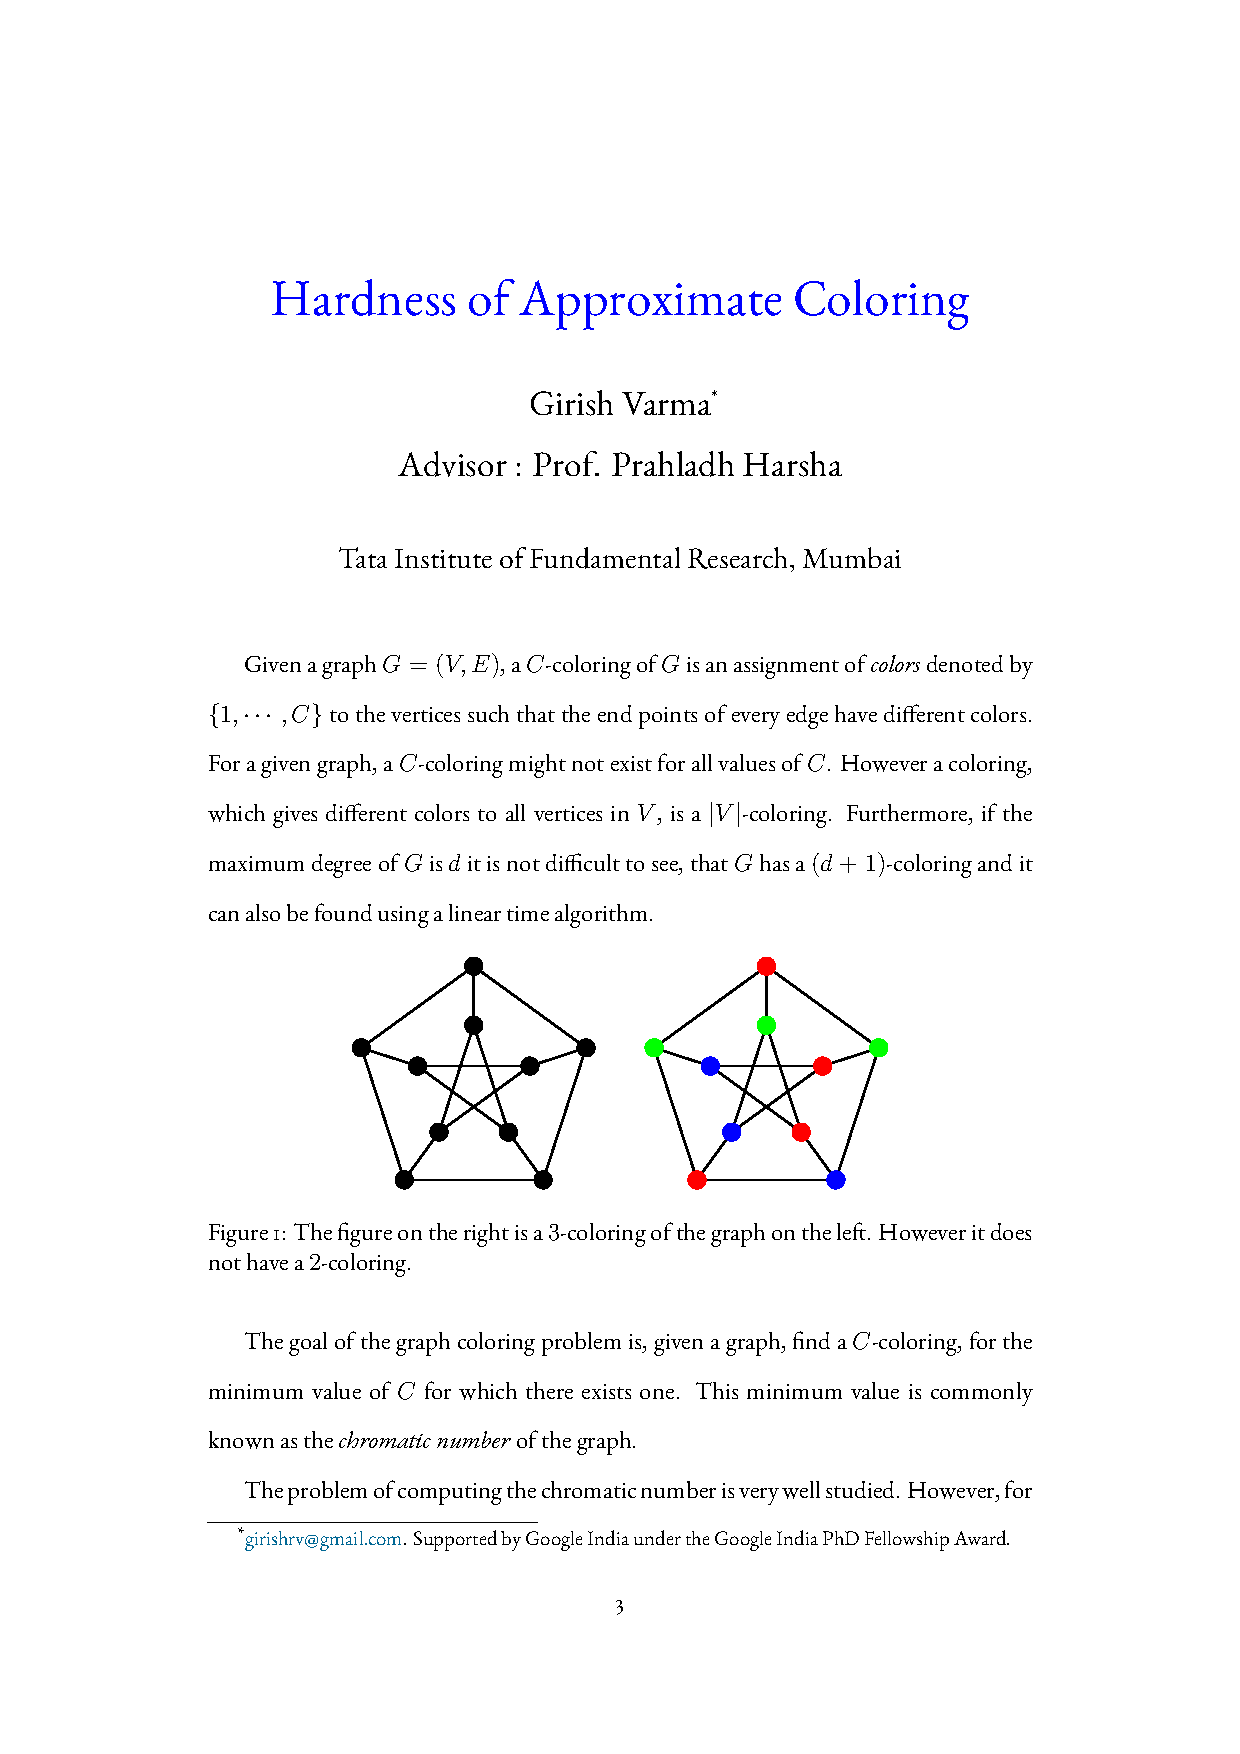
\includepdf[pages=-]{synopsis.pdf}

\part*{\sc Thesis}
\cleardoublepage
\addcontentsline{toc}{part}{\sc B\quad Thesis}
\fi
\begin{savequote}[75mm] 
Simple can be harder than complex: You have to work hard to get your thinking clean to make it simple. But it’s worth it in the end because once you get there, you can move mountains. 
\qauthor{Steve Jobs} 
\end{savequote}
\chapter*{}

\part{Introduction}\label{part:one}

\setcounter{chapter}{0}  


\chapter{Puzzles, Algorithms \& Hardness} 


\label{ch:puzz-algo-hard}
\section{Coloring Puzzle}

\begin{figure}[h] \label{fig:graph}
\centering 
\begin{tikzpicture}[style=thick] 
\draw (18:2cm) -- (90:2cm) -- (162:2cm) -- (234:2cm) -- (306:2cm) -- cycle;
\draw (18:1cm) -- (162:1cm) -- (306:1cm) -- (90:1cm) -- (234:1cm) -- cycle;
\foreach \x in {18,90,162,234,306}{ 
	\draw (\x:1cm) -- (\x:2cm); 
}
\draw[fill=black] (18:2cm) circle (4pt);
\draw[fill=black] (90:2cm) circle (4pt);
\draw[fill=black] (90:1cm) circle (4pt); 
\draw[fill=black] (18:1cm) circle (4pt); 
\draw[fill=black] (162:1cm) circle (4pt); 
\draw[fill=black] (162:2cm) circle (4pt); 
\draw[fill=black] (234:1cm) circle (4pt);
\draw[fill=black] (234:2cm) circle (4pt); 
\draw[fill=black] (306:1cm) circle (4pt); 
\draw[fill=black] (306:2cm) circle (4pt);
\end{tikzpicture} 
\end{figure}

Consider the following puzzle. Given a figure
as above, the goal is to give colors to the circles such that
for every line, its end points have different colors. Furthermore, the number of
colors used needs to be minimized. Without this condition the problem is
trivial since using a different color for every circle would be a solution
irrespective of the figure.

Puzzles like above are very commonly encountered in a variety of real life
instances. However known algorithms takes far too much time to complete even on
instances with $20$ vertices. This thesis is about an explanation for the
lack of efficient algorithms, for coloring like problems.

\begin{figure}[h] 
\centering 
\begin{tikzpicture}[style=thick] 
\draw (18:2cm) -- (90:2cm) -- (162:2cm) -- (234:2cm) -- (306:2cm) -- cycle;
\draw (18:1cm) -- (162:1cm) -- (306:1cm) -- (90:1cm) -- (234:1cm) -- cycle; 
\foreach \x in {18,90,162,234,306}{ \draw (\x:1cm) -- (\x:2cm); }
\draw[fill=black] (18:2cm) circle (4pt); 
\draw[fill=black] (90:2cm) circle (4pt); 
\draw[fill=black] (90:1cm) circle (4pt); 
\draw[fill=black] (18:1cm) circle (4pt); 
\draw[fill=black] (162:1cm) circle (4pt); 
\draw[fill=black] (162:2cm) circle (4pt); 
\draw[fill=black] (234:1cm) circle (4pt);
\draw[fill=black] (234:2cm) circle (4pt); 
\draw[fill=black] (306:1cm) circle (4pt); 
\draw[fill=black] (306:2cm) circle (4pt);
\end{tikzpicture} 
\qquad \qquad  
\begin{tikzpicture}[style=thick] 
\draw (18:2cm) -- (90:2cm) -- (162:2cm) -- (234:2cm) -- (306:2cm) -- cycle; 
\draw (18:1cm) -- (162:1cm) -- (306:1cm) -- (90:1cm) -- (234:1cm) -- cycle; 
\foreach \x in {18,90,162,234,306}{ 
	\draw (\x:1cm) -- (\x:2cm); 
}
\draw[color=green,fill=green] (18:2cm) circle (4pt); 
\draw[color=red,fill=red] (90:2cm) circle (4pt); 
\draw[color=green,fill=green] (90:1cm) circle (4pt);
\draw[color=red,fill=red] (18:1cm) circle (4pt); 
\draw[color=blue,fill=blue] (162:1cm) circle (4pt); 
\draw[color=green,fill=green] (162:2cm) circle (4pt);
\draw[color=blue,fill=blue] (234:1cm) circle (4pt); 
\draw[color=red,fill=red] (234:2cm) circle (4pt); 
\draw[color=red,fill=red] (306:1cm) circle (4pt);
\draw[color=blue,fill=blue] (306:2cm) circle (4pt); 
\end{tikzpicture}
\caption{The figure on the right is a $3$-coloring of the graph on the left.
However it does not have a $2$-coloring.} 
\label{fig:M1} 
\end{figure} 
Figures
like above are commonly called \emph{graphs}
 (strictly speaking they are undirected graphs, but in this thesis will
 only be concerned with undirected graphs) . A graph $G=(V,E)$ consists of a
set of \emph{vertices} $V$ (the circles) and a set $E$ containing some pairs of
vertices, called \emph{edges} (the lines).

Given a graph $G=(V,E)$ and a number $C$, a $C$-coloring of $G$ is an assignment
of \emph{colors} denoted by $\{1,\cdots, C\}$ to the vertices such that the end
points of every edge have different colors. For a given graph, a $C$-coloring
might not exist for all values of $C$. But for any graph, the coloring which
gives different colors to all vertices in $V$, is an $n$-coloring, where $n$ is
the \emph{size} (the number of vertices in $V$) of $G$.

\begin{definition} The \GraphColoring\ problem is, given a graph, find a
coloring, using the minimum number of colors. This
minimum value is commonly known as the \emph{chromatic number} of the graph.
\end{definition}

\section{Efficient Algorithms}

If the maximum degree of $G$ is $\Delta$ then the following simple algorithm computes
a $(\Delta+1)$-coloring in time bounded by the number of edges.
\paragraph{}
\begin{algorithm}[H] 
\caption{For graphs with maximum degree $\leq\Delta$.} 
\For{$v \in V$}{ 
	give $v$ a color in $\{1,\cdots,\Delta+1\}$ different from the colors of its
	already colored neighbours.
} 
\end{algorithm}
\qquad

Algorithm 1, does not solve the \GraphColoring\ problem since the chromatic
number can be much smaller than $\Delta+1$.
Suppose the graph has a $c$-coloring there is a simple algorithm to find it,
which takes $c^n\cdot m$ time, where $m$ is the number of edges.
\paragraph{}
\begin{algorithm}[H] 
\label{alg:brut} 
\caption{Brute Force Algorithm} 
\For{every assignment $f \in \{1,\cdots,c\}^V$ of colors to the vertices }{ 
	\For{every edge}{
		check if $f$ assigns different colors to the end points.
	} 
}
\end{algorithm}
\qquad

However note that the running time of Algorithm 2 grows
\emph{exponentially} in $n$. Even for $n=20$, the running time ($> c^{20}$) is
prohibitively large, while for Algorithm 1 it is still a reasonable number. This
motivates the definition of efficient algorithms, as ones that has running time
bounded by a polynomial in the input size. For simplicity, we consider only
\emph{decision problems} (\ie problems that have a Boolean answer). For such
problems the inputs are partitioned into YES and NO instances. We will often
specify a decision problem by the set of YES instances. Though \GraphColoring\
problem is not a decision problem, we can consider the problem which have the
number $C$ also in the input, where the goal is to check if the graph has a
$C$-coloring. 
%TODO: Motivate and give references for efficient = polytime

\begin{informal-definition}\label{def:p} 
\P\ is the class of decision problems, that has an algorithm
with running time bounded by a polynomial in $n$ (the input size).
\end{informal-definition}

Note that for \GraphColoring, $(G,C) \in \YES$ (i.e. $G$ has a $C$-coloring),
then there is a certificate that certifies that it is \YES\ instance, that can
be verified in time proportional to the number of edges. The certificate is
simply the $C$-coloring of the graph. And if $(G,C) \in \NO$, then any assignment
of colors from $\{1,\cdots, C\}$, will leave some edge monochromatic. This
property is true for a large class of problems.

\begin{informal-definition} \label{def:np}
 \NP\ is the class of decision problems, for which there is an
algorithm $V$ which takes an input $x$ and a proof $\pi$, runs in time
polynomial in the size of $x$ and satisfies the following properties.
\begin{itemize} 
\item Completeness : If $x \in \YES$ then there exists $\pi$
such that $V(x,\pi)=1$. 
\item Soundness : If $x\in \NO$ then for any $\pi$,
$V(x, \pi)=0$. 
\end{itemize} 
\end{informal-definition}

For any \NP\ problem, there is a trivial algorithm similar to Algorithm
\ref{alg:brut}, which runs in time $c^n$ for some constant $c$. The algorithm
just tries all possible certificates with the verification procedure. It is a
major open problem if \P $=$ \NP. A surprising result is that there are certain
class of problems called \NPComplete\ which capture the hardness of solving
problems in \NP. That is, an instance of any \NP\ problem could be converted
efficiently to an instance of such problems. 
The \GraphColoring\ problem is an \NPComplete\ problem. Hence unless $\P = \NP$,
we cannot hope to have polynomial time algorithms for \GraphColoring. One can
ask if there are polynomial time algorithms for a relaxed version of the
problem.

\section{Approximation Algorithms} 
\label{sec:approx} 
A relaxed
version of the \GraphColoring\ problem is to compute the chromatic number
approximately. An \emph{approximation algorithm} for chromatic number with
approximation \emph{factor} $F \geq 1$, always outputs a number between $C$ and
$C\cdot F$, where $C$ is the chromatic number of the input graph.
 
However for a general graph, this relaxation is also a \emph{hard} problem. That
is, assuming the famous $\P\neq \NP$ conjecture, it is known that this problem
cannot be solved in polynomial time. Feige \& Kilian~\cite{FeigeK00} showed that
computing this number approximately within a factor of $n^{1-\epsilon}$ for any
small constant $\epsilon >0$ is known to be  hard, assuming a different complexity
conjecture. Therefore, there is not much hope of having an efficient algorithm,
which does much better than the trivial $n$-coloring.

Since the general approximation problem is hard, the focus shifted on solving it
for subclasses of graphs. A natural subclass of graphs to consider, are the ones
for which the chromatic number is a small constant $c$. For $c=2$, such graphs
are commonly called \emph{bipartite}. There is a simple linear time algorithm
for finding a $2$-coloring in such graphs. It just assigns a vertex one color,
the other color to all its neighbours, and continues until all vertices are
colored. However for $3$-colorable graphs, finding a $3$-coloring is \NPHard\
(it cannot be solved by efficient algorithms, assuming \P$\neq$ \NP).

Hence a long series of works, was aimed at solving this problem approximately.
\begin{definition} 
\ApproximateGraphColoring$(c,C)$ problem is to find a
$C$-coloring, when the input graph is promised to be $c$-colorable.
\end{definition} 

\begin{remark}
We will often be considering the decision version of the problem, specified by
disjoint sets of \YES\ ($c$-colorable graphs) and \NO\ (graphs with chromatic
number $> C$) instances. The goal is to have an algorithm to accept all \YES\
instances and reject all \NO\ instances. The algorithm can either accept 
or reject inputs which are neither \YES\ nor \NO. 
\end{remark}

For $3$-colorable
graphs, Wigderson~\cite{Wigderson83} gave the first not trivial improvement of
finding a $O(\sqrt n)$-coloring using combinatorial techniques. This was further
improved to $O(n^{3/8})$-coloring by Blum~\cite{Blum94}. A major breakthrough
 was made by Karger, Motwani \&
Sudan~\cite{KargerMS1998}, using semi-definite programming (SDP). For a
$3$-colorable graph with maximum degree $d$, they gave an $O(d^{1/3})$-coloring
algorithm. Combining this with Wigderson's algorithm, they obtained a
$O(n^{1/4})$-coloring algorithm. Blum \& Karger~\cite{BlumK1997} combined the
combinatorial methods of Blum~\cite{Blum94} with the SDP to get an
$O(n^{3/14})$-coloring. The current best known (see results of Kawarabayashi \& Thorup
\cite{KawarabayashiT2014}) efficient algorithms output a $n^{0.19996}$-coloring.


\section{What this thesis is about?}

This thesis is about giving an explanation for the lack of efficient algorithms for
some generalizations of the \ApproximateGraphColoring$(c,C)$ problem, 
using the theory of \NPComplete ness and complexity conjectures similar 
to \P $\neq$ \NP. That is, we prove that efficient algorithms for the problem
will imply that the corresponding conjecture is false.  
Such results are called \emph{hardness 
results} and the area in general, is commonly called in literature as
the \emph{hardness of approximation}. The focus of our hardness
results will be the case when $c$ is a small constant and $C$ can be 
any large constant or a function that depends on $n$. 
As described in the previous section,
there are algorithms which solve these problems for $C=n^\alpha$ for
some constant $\alpha <1$. We prove hardness results for larger values
(exponentially larger in some cases)
of $C$ than was previously known. 
We will describe these generalizations in the next three sections.

\subsection{Almost Coloring}

Assuming \P$\neq$ \NP, Khanna \etal~\cite{KhannaLS2000}
showed hardness for the \ApproximateGraphColoring$(3,4)$ problem
 (that is there is no efficient algorithm which can find a $4$-coloring,
 in any $3$-colorable graph). Since then, there has been no progress
 in  this problem. Later, results where proved using a complexity
  assumption called the Unique Games Conjecture (UGC), 
  which is stronger than the P$\neq$ NP assumption.
Starting with the work of Khot~\cite{Khot2002}, it was shown that  
UGC, explains the lack of efficient approximation algorithms for a 
variety of problems (eg. Vertex Cover, MAX-CUT).
 Dinur, Mossel \& Regev~\cite{DinurMR2009} showed hardness for
 \ApproximateGraphColoring$(3,C)$ for any constant $C$ using
 a conjecture similar to \UGC. Due to a technical problem (that
 \UGC\ does not have perfect completeness), their results which
 used \UGC\ exactly, showed hardness for the 
 \AlmostGraphColoring{\epsilon}$(c,C)$ problem, for any small
 $\epsilon >0$.
 \begin{definition}
 The \AlmostGraphColoring{\epsilon}$(c,C)$ problem is
 of distiguishing graph from the following cases:
 \begin{itemize}
 \item \YES\ : There is a subgraph of size $(1-\epsilon)n$ that is 
 $c$-colorable.
 \item \NO\ : Any independent set is the graph has size at most $n/C$.
 \end{itemize}
 \end{definition}
 \noindent
 \paragraph{\underline{Contributions of this Thesis:}}	
The work of Dinur \& Shinkar~\cite{DinurS2010} 
implies hardness results for \AlmostGraphColoring{\epsilon}$(3,\poly(\log n))$,
 using a stronger form of \UGC\ (where the dependence
 between the soundness and alphabet size is inverse polynomial).
In \lref[Chapter]{ch:graph-hard}, we show hardness for 
the same problem, using a weaker form of UGC (in which the 
aforesaid dependence 
is super-polynomial) in some respects (joint work with Dinur, Harsha \& Srinivasan~\cite{DinurHSV2014}).

The previous reductions (by Dinur, Mossel \& Regev~\cite{DinurMR2009}
and Dinur \& Shinkar~\cite{DinurS2010}) followed
the template of H\aa stad \cite{Hastad2001}, which employed a particular
error correcting code known as the long code. As the name implies, this
code has a large size which made the reductions inefficient. A shorter
code called the low degree long code was proposed by 
Barak \etal~\cite{BarakGHMRS2012} . Dinur and Guruswami~\cite{DinurG2013} showed
improved approximate covering (which we define in \lref[Section]{sec:intro-cover}) hardness results 
 using this shorter code. In \lref[Chapter]{ch:graph-hard}, we  adapt this shorter code
  to the reduction of Dinur, Mossel and Regev~\cite{DinurMR2009} for graph coloring,
  to get improved results.
 
 

 
  %Mention results of Sion Chan, Sanxia Huang, Khot, DinurMR, DS on graph coloring hardness
 

\subsection{Hypergraph Coloring}		

Guruswami, H\aa stad \& Sudan~\cite{GuruswamiHS2002} initiated
the study of hypergraph coloring problems, to
get a better understanding of graph coloring and since it
is a natural generalization. They showed
hardness results for $c=2, C=\poly(\log \log n)$, for hypergraph coloring, 
assuming
that \NP\ does not have quasi-polynomial algorithms (such
results are commonly known as \emph{quasi-\NP-hardness} results). 
A
\emph{$k$-uniform hypergraph} $G=(V,E)$ is similar to a graph, with the edges
$E\subseteq {V \choose k}$ containing $k$ vertices. A $c$-coloring of a hypergraph is
coloring of vertices using colors $\{1,\cdots, c\}$, such that every edge
has $2$ vertices with distinct colors. For $k=2$,
a hypergraph is simply a graph. 
%TODO: Strictly speaking this is not a generalization since all vertices in an edge 
% may not be distinct. But the proofs also holds for undirected versions. 
\begin{definition} 
The \ApproximateHypergraphColoring{k}$(c,C)$ problem is defined similar to
\ApproximateGraphColoring$(c,C)$, as given a $c$-colorable $k$-uniform
hypergraph, find a $C$-coloring. The decision version is also defined
analogously. 
\end{definition}
When $k>2$, for any constant $c>1$, known algorithms only guarantee an
 $n^\alpha$-coloring for some $\alpha < 1$. Starting
 with the work of Guruswami, H\aa stad \& Sudan \cite{GuruswamiHS2002}, 
 there have been many results in hardness of hypergraph coloring.
 For the case of constant $c,k$, strongest known results 
 due to Khot~\cite{Khot2002c}, who showed 
quasi-\NP-hardness  for $C= \poly( \log n)$.
\noindent
\paragraph{\underline{Contributions of this Thesis:}}
In \lref[Chapter]{ch:hypergraph-hard}, we exponentially improve the hardness
results.  In \lref[Section]{sec:33}, we first show hardness results (joint work with Guruswami, Harsha, H\aa stad \& 
Srinivasan~\cite{GuruswamiHHSV2014}) for 
$3$-uniform $3$-colorable hypergraphs by a more efficient reduction,
that makes use of low degree long code (which we describe in \lref[Section]{sec:low-deg-long-code}).
For the case of $4$-uniform $4$-colorable hypergraphs, 
our initial work (joint work with Guruswami, Harsha, H\aa stad \& 
Srinivasan~\cite{GuruswamiHHSV2014}) showed the first
super-polylogarithmic coloring hardness (i.e. $C >> \poly(\log n)$)  results, by
using the low degree long code. 
Subsequent to our initial work Khot \&
Saket~\cite{KhotS2014b} got hardness results of $2^{(\log
n)^{1/21}}$, by using the low degree long code with degree $2$. Though their result was
for $12$-uniform hypergraphs. We further observed~\cite{Varma2014} that
by combining their methods with ours, the same hardness results can be
obtained for $4$-uniform hypergraphs. Hence  we improved the hardness
results from $\poly(\log n)$ to $2^{(\log n)^{1/21}}$ for
the case of $4$-colorable $4$-uniform hypergraphs. 

\subsection{Covering CSPs}
\label{sec:intro-cover}
The covering problem for constraint satisfaction~(CSP) is a generalization of the hypergraph
coloring problem, introduced by
Guruswami, H\aa stad and Sudan~\cite{GuruswamiHS2002} and later studied in 
detail by Dinur \& Kol~\cite{DinurK2013}. An instance of the problem
consists of a hypergraph $G=(V,E)$ along with a \emph{predicate} $P
\subseteq \{0,1\}^k$ and a \emph{literal} function $L:E\rightarrow
\{0,1\}^k$. An \emph{assignment} $f:V \rightarrow \{0,1\}$
\emph{covers} an edge $e\in E$, if $f|_e \oplus L(e) \in P$ (by $f|_e$,
we mean the $k$ bit string, obtained by restricting $f$ to vertices in $e$, and the 
$\oplus$ operation is coordinate-wise parity of the two strings). 
A \emph{cover} for a CSP instance is a set of 
assignments such that every edge is covered by one of the assignments.
 The goal of the covering problem is to find the minimum sized cover.
 
 When the predicate is the $3$-OR predicate, we can view the
 instance as a $3$-SAT instance, where each edge is a clause and the literal function
 specifies which variables are to be negated.
 Then the satisfiability problem is equivalent to finding a cover of size $1$.
The covering problem can also be thought of as a generalization of the coloring
problem. Consider an instance $G$  with the NAE(
$:=\{0,1\}^k \setminus \{ \overline 0, \overline 1\}$) predicate 
and the trivial literal function $L(e) = 0^k$ for every edge $e$.
It is not difficult to see that $G$ has a cover of size $t$
 iff $G$ is $2^t$-colorable. The \emph{approximate covering} problem is defined as,
given a $c$-coverable instance, find a $C$-covering.\\
\begin{definition}[\cov-$P$-\csp$(c,C)$]
  
	\label{def:cov-csp}
	For $P \subseteq \setq^k$ and $c,C \in \nat$, the \cov-$P$-\csp$(c,C)$ problem is, 
	given a $c$-coverable instance  $(G=(V,E),L)$ of $P$-\csp, find an 
	$C$-covering.
\end{definition}

A predicate $P$ is \emph{odd}, if for every $x \in \{0,1\}^k$ either $x \in
P$ or $\overline{x} \in P$. For odd predicates,
there is a trivial algorithm with factor $2$, since any assignment
and its complement covers the CSP instance. Dinur \& Kol~\cite{DinurK2013} asked the question
whether,  the approximate covering problem is hard for any constant $C>c$, for all non-odd
predicates. Assuming a variant of UGC, they proceeded to show that if a non-odd predicate has a
pairwise independent distribution in its support then, this is indeed
the case.


\noindent
\paragraph{\underline{Contributions of this Thesis:}}
In \lref[Chapter]{ch:covering-hard}, we answer the question of Dinur \& Kol in the affirmative 
(joint work with Bhangale \& Harsha~\cite{BhangaleHV2014}). That is,
the approximate covering problem for a non-odd predicate is hard for any constant $C>c$ 
(assuming the same conjecture as Dinur \& Kol used). 
This leads to a complete characterization of predicates for which this result can be true,
since there is a trivial $2$-covering algorithm for odd predicates. 
Our results also holds over non binary alphabets. 
We also show NP-hardness results, for the approximate covering problem with parameters
$c=2, C = \log \log n$, for a class of predicates. Previously such results were  known due to
Dinur \& Kol  for $4$-LIN with $c=2,C= \log \log \log n$.




\section{Organization of Thesis} 

This thesis has two main parts. In
\lref[Part]{part:two}, we will introduce some of the mathematical techniques
used in proving the hardness results. \lref[Part]{part:three} contains all the
hardness results.

In \lref[Part]{part:two}, we also prove some lemmas which form the
basis of the results in the next part. In \lref[Chapter]{ch:harmonic}, 
\lref[Section]{sec:har-poly} is a contribution of this thesis, were we 
prove analogues of results in Boolean function analysis to functions
on subspaces. 
In \lref[Chapter]{ch:testing}, we discuss
a linear algebraic result about testing low degree polynomials.
\lref[Section]{sec:square-test} is a contribution of this thesis,
though the analysis is similar to the results of Dinur \&
Guruswami~\cite{DinurG2013} mentioned in \lref[Section]{sec:prod-test}. In
\lref[Chapter]{ch:graph-prod}, we also give some combinatorial results about
derandomized graph products. \lref[Section]{sec:derand-graph-prod} and
\lref[Section]{sec:derand-maj-stab} are contributions of this thesis
which uses the results proved in \lref[Section]{sec:square-test}.

\lref[Part]{part:three} contains all the hardness results about almost graph 
coloring (\lref[Chapter]{ch:graph-hard}; joint work with Dinur, Harsha \& Srinivasan~\cite{DinurHSV2014}), hypergraph coloring
(\lref[Chapter]{ch:hypergraph-hard}; joint work with Guruswami, Harsha, H\aa stad \& 
Srinivasan~\cite{GuruswamiHHSV2014} and the result \cite{Varma2014} ), and covering problem
(\lref[Chapter]{ch:covering-hard}; joint work with Bhangale \& Harsha~\cite{BhangaleHV2014}). These results are the main contributions of
this thesis, though much of the hardness reductions and analysis are similar to
previous works.



\part{Mathematical Techniques}\label{part:two}



\chapter{Analysis of Functions on Product Spaces}

In this chapter, we will describe some results concerning functions
on product probability spaces.

\section{Preliminaries}

Let $(\Omega, \mu)$ be a discrete probability space and
$(\Omega^L,\mu^{\otimes L})$ be the corresponding product space. For a function
$f:\Omega^L \rightarrow \R$, the \emph{Efron-Stein decomposition} of $f$ with
respect to the product space is given by
$$ f(x_1,\cdots, x_L) = \sum_{\beta \subseteq [L]} f_\beta(x),$$
where $f_\beta$ depends only on $x_i$ for $i\in \beta$ and 
$$ \forall \beta' \not\supseteq \beta , a \in \Omega^{\beta'}, \E_{x \in
\mu^{\otimes L}} \left[ f_\beta(x) \mid x_{\beta'} = a \right]=0.$$
The $\ell_p$ and $\ell_\infty$ norms of $f$ with respect to the probability space
are defined as
$$\|f\|_p := \E_{x\in \mu^{\otimes L}}\left[f(x)^p\right]^{1/p},
~~~~~~~~~~~~\|f\|_\infty :=\max_{x\in \Omega^{\otimes L}}\left|f(x)\right|.$$ 
For $i \in [L]$, the \emph{influence} of the $i$th
coordinate on $f$ is defined as follows.
$$\Inf_i[f] := \E_{x_1,\cdots, x_{i-1},x_{i+1},\cdots , x_L}\Var_{x_i}[f
(x_1,\cdots, x_L)]  = \sum_{\beta: i\in \beta} \|f_\beta\|^2_2.$$
For an integer $d$, the \emph{degree $d$ influence} is defined as
$$\Inf_i^{\leq d}[f] := \sum_{\beta: i\in \beta, |\beta| \leq d} \|f_\beta\|^2_2.$$

\section{Invariance Principle}
%TODO: Motivate Invariance Principle More

Let $(\Omega^k, \mu)$ be a probability space. Let $\supp(\mu) := \{ x\in \Omega^k 
\mid \mu(x) > 0\}$. 

\begin{definition}[Connected Sets and Distributions] \label{def:connected}
We say that  $S \subseteq \Omega^k$ is 
\emph{connected} if for every $x, y\in S$, there is a sequence of strings 
starting with $x$ and ending with $y$ such that every element in the sequence is
in $S$ and every two adjacent elements differ in exactly one coordinate. 
The probability space is connected if $\supp(\mu)$ is connected.
\end{definition}


\begin{theorem}[{Mossel~\cite[Proposition 6.4]{Mossel2008}}]

	\label{thm:invariance}
	Let $(\Omega^k, \mu)$ be a connected probability space such the minimum probability of
	every atom in $\supp(\mu)$ is at least $\alpha \in \left(0, \frac{1}{2}\right]$.
	 Then there exists 
	continuous functions $\overline{\Gamma} : (0,1)\rightarrow (0,1)$ and 
	$\underline{\Gamma} : (0,1)\rightarrow (0,1)$ such that the following holds: 
	For every $\epsilon>0$, there exists $\tau > 0$ and an integer $d$ such that 
	if a function $f : \Omega^L \rightarrow [0,1]$ satisfies
	%
	$$\forall i\in [n],  \Inf_i^{\leq d} (f) \leq \tau $$
	%
	then 
	%
	$$\underline{\Gamma}\left(\E_\mu[f]\right) -\epsilon \leq \E_{(x_1,\ldots, x_k) \sim \mu}\left[
	\prod_{j=1}^k f(x_j)\right] \leq \overline{\Gamma}\left(\E_\mu[f]\right) + \epsilon.$$
	%
	There exists an absolute constant $C$ such that one can take $\tau = \epsilon^
	{C\frac{\log(\nicefrac{1}{\alpha})\log(\nicefrac{1}{\epsilon})}{\epsilon
	\alpha^2}}$ and $d = \log(\nicefrac{1}{\tau})\log(\nicefrac{1}{\alpha})$.
\end{theorem}

Correlation is a measure of dependence in probability spaces where the sample space
is a product set.

\begin{definition}[Correlated Spaces]
\label{def:correlation}
Let $(\Omega_1 \times \Omega_2, \mu)$ be a finite probability space, the correlation between $\Omega_1$ and $\Omega_2$ with respect to $\mu$ us defined as 
$$\rho(\Omega_1, \Omega_2; \mu) := \mathop{\max}_{\substack{f : \Omega_1 \rightarrow \R, \E[f]  = 0 , \E[f^2]\leq 1 \\ g: \Omega_2 \rightarrow \R, \E[g] = 0 , \E[g^2]\leq 1} }  \E_{(x,y) \sim \mu }[ |f(x)g(y)|] .$$
For a probability space $\left(\prod_{i=1}^k\Omega_i, \mu\right)$, the correlation is given by
$$\rho\left(\prod_{i=1}^k\Omega; \mu\right) := \max_{i \in [k]} \rho\left( \Omega_i, \prod_{ j \in [k], j \neq i} \Omega_i; \mu\right).$$ 
\end{definition}

The following result about correlated spaces is an
adaptation of similar results (see Wenner
\cite[Theorem~3.12]{Wenner2013} and Guruswami \& 
Lee~\cite[Lemma~A.1]{GuruswamiL2015})   to proving
our hardness results.
 
\begin{theorem}

  \label{thm:inv-prin} Let $(\Omega_1^k \times \Omega_2^k, \mu)$ be a
  correlated probability space with correlation $\rho < 1$
   such that the marginal of $\mu$ on any
  pair of coordinates one each from $\Omega_1$ and $\Omega_2$ is a
  product distribution. Let $\mu_1 ,\mu_2$ be the marginals of $\mu$
  on $\Omega_1^k$ and $\Omega_2^k$ respectively. Let $X, Y$ be two
  random $k\times L$ dimensional matrices chosen as follows:
  independently for every $i \in [L]$, the pair of columns $(x^i,y^i)
  \in \Omega_1^k \times \Omega_2^k$ is chosen from $\mu$. Let
  $x_i,y_i$ denote the $i$\th rows of $X$ and $Y$ respectively.  If
  $F: \Omega_1^L \rightarrow [-1,+1]$ and $G: \Omega_2^L \rightarrow
  [-1,+1]$ are functions such that
	$$\tau:= \sqrt{\sum_{i \in [L]}\Inf_i[F]\cdot \Inf_i[G]}  ~\text{ and } ~
	\Gamma := \max \left\{ \sqrt{\sum_{i \in [L]}\Inf_i[F]} , \sqrt{\sum_{i \in 
	[L]}\Inf_i[G]} \right\} \ ,$$ then
		\begin{equation}
		\label{eqn:inv-eqn}
		\abs{ \E_{(X,Y) \in \mu^{\otimes L}} \left[\prod_{i\in [k]}F(x_i) G(y_i)
		\right] - \E_{X \in \mu_1^{\otimes L}} \left[\prod_{i\in [k]}F(x_i)\right]
		\E_{Y \in \mu_2^{\otimes L}} \left[\prod_{i\in [k]}G(y_i)\right] } \leq 
		2^{O(k)} \Gamma \tau.
	\end{equation}
\end{theorem}

\begin{proof}

	We will prove the theorem by using the hybrid argument. For $i \in [L+1]$, let 
	$X^{(i)},Y^{(i)}$ be distributed according to $(\mu_1 \otimes \mu_2)^{\otimes
	 i} \otimes \mu^{\otimes L- i}$. Thus, $(X^{(0)},Y^{(0)}) =
       (X,Y)$ is distributed according to $\mu^{\otimes L}$ while
       $(X^{(L)},Y^{(L)})$ is distributed according to
       $(\mu_1\otimes\mu_2)^{\otimes L}$. For $i \in [L]$, define
	%
	\begin{equation}
		\label{eqn:err}
		\err_i := \abs{ \E_{X^{(i)},Y^{(i)}} \left[\prod_{j=1}^kF(x^{(i)}_j) 
		G(y^{(i)}_j)\right] - \E_{X^{(i+1)},Y^{(i+1)}} \left[\prod_{j=1}^kF(x^
		{(i+1)}_j) G(y^{(i+1)}_j)\right] }.
	\end{equation}
%
	The left hand side of Equation \eqref{eqn:inv-eqn} is upper bounded by $\sum_{i\in [L]} 
	\err_i$.  Now for a fixed $i$,  we will bound $\err_i$. We use the 
	Efron-Stein decomposition of $F,G$ to split them into two
        parts: the part which depends on the 
	$i$th input and the part independent of the $i$th input. 
	%
	$$F= F_0 + F_1 \text{ where } F_0 := \sum_{\alpha : i\notin \alpha} F_\alpha \mbox{ and } 
	F_1 := \sum_{\alpha : i\in \alpha} F_\alpha.$$
	%
	$$G = G_0 + G_1 \text{ where } G_0 := \sum_{\beta : i\notin \beta} G_\beta  \mbox{ and } 
	G_1 := \sum_{\beta : i\in \beta} G_\beta.$$
	%
	Note that $\Inf_i[F] = \|F_1\|^2_2$ and $\Inf_i[G] =
        \|G_1\|_2^2$. Furthermore, the functions $F_0$ and $F_1$ are
        bounded since $F_0(x) = \E_{x^{'}} [F(x^{'}) |
        x^{'}_{[L]\setminus i} = x_{[L]\setminus i} ] \in [-1,+1]$ and
        $F_1(x) = F(x) - F_0(x) \in [-2,+2]$.  For $a \in \{0,1\}^k$,
        let $F_a(X) := \prod_{j =1}^kF_{a_j}(x_j)$.  Similarly
        $G_0,G_1$ are bounded and $G_a$ defined
        analogously. Substituting these definitions in Equation
        \eqref{eqn:err} and expanding the products gives
	% 
	$$\err_i = \abs{ \sum_{a,b \in \{0,1\}^k}\left(  \E_{X^{(i)},Y^{(i)}} 
	\left[F_{a}(X^{(i)}) G_{b}(Y^{(i)})\right]  - \E_{X^{(i+1)},Y^{(i+1)}} \left[
	F_{a}(X^{(i+1)}) G_{b}(Y^{(i+1)})\right]  \right) }.$$
	%
	Since both the distributions are identical on
	$(\Omega_1^k)^{\otimes L}$ and $(\Omega_2^k)^{\otimes L}$, all
	terms with $a = \bar 0$ or $b=\bar 0$ are zero. Because $\mu$
	is uniform on any pair of coordinates on each from the
	$\Omega_1$ and $\Omega_2$ sides, terms with $|a|=|b|=1$ also
        evaluates to zero. Now consider the remaining terms with $ |a|,|b| \geq1,
	|a|+|b| > 2$. Consider one such term where $a_{1},a_2 = 1$ and $b_{1}
	=1$. In this case, by Cauchy-Schwarz inequality we have that
	%
	\begin{align*}
	\begin{split}
		\abs{ \E_{X^{(i-1)},Y^{(i-1)}} \left[F_a(X^{(i-1)}) G_{b}(Y^{(i-1)})\right]}
		 \leq &\sqrt{\E F_1(x_1)^2 G_1(y_1)^2}  \\ &\cdot \|F_1\|_2  \cdot \left\| 
		\prod_{j>2} F_{a_j}\right\|_\infty \cdot \left\| \prod_{j> 1} G_{b_j}\right
		\|_\infty.
	\end{split}
	\end{align*}
	From the facts that the marginal of $\mu$ to any pair of
	coordinates one each from $\Omega_1$ and $\Omega_2$ sides are
	uniform, $\Inf_i[F] = \|F_1\|_2^2$ and
	$|F_0(x)|,|F_1(x)|,|G_0(x)|,|G_1(x)|$ are all bounded by $2$,
	the right side of above becomes
		\begin{align*}
 \sqrt{\E F_1(x_1)^2} \sqrt{\E G_1(y_1)^2} \cdot \|F_1\|_2  \cdot \left\|
		\prod_{j>2} F_{a_j}\right\|_\infty \cdot \left\| \prod_{j> 1} G_{b_j}
		\right\|_\infty \leq  \sqrt{\Inf_i[F]^2 \Inf_i[G]} \cdot 2^{2k} .
	\end{align*}
	%
	All the other terms corresponding to other $(a,b)$ which are
	at most $2^{2k}$ in number, are bounded analogously. Hence,
	%
	\begin{align*}
		\sum_{i \in [L]} \err_i &\leq 2^{4k} \sum_{i \in [L]} \left( \sqrt{\Inf_i[F]
		^2\Inf_i[G]} +\sqrt{\Inf_i[F]\Inf_i[G]^2} \right)\\
		 &= 2^{4k} \sum_{i \in [L]} \sqrt{\Inf_i[F]
		\Inf_i[G]}\left( \sqrt{\Inf_i[F]} +\sqrt{\Inf_i[G]} \right).
	\end{align*}
By	applying the Cauchy-Schwarz inequality, followed by a triangle inequality, we obtain	
 	\begin{align*}
		\sum_{i \in [L]} \err_i&\leq 2^{4k} \sqrt{\sum_{i \in [L]} \Inf_i[F]\Inf_i[G]}\left(\sqrt{\sum_{i \in [L]}  \Inf_i[F]} + \sqrt{\sum_{i \in 
		[L]}  \Inf_i[G]} \right).
	\end{align*}
Thus, proved.
\end{proof}





\chapter{Harmonic Analysis of Functions}
\label{ch:harmonic}

In this chapter, we describe some tools for analyzing functions over probability
spaces, for which the sample space exhibits a field structure, and the 
distribution is defined in terms of the field operations.  In this case, we can 
obtain decompositions with special properties, that helps in 
analysing such distributions. We will be concerned with
the sample space which is the vector space of functions of the 
form $f:\F_p^R \rightarrow \F_p$ ($p$ is a prime).
 We  extend these decompositions and the associated results
 to the case when the domain is the subspace of low degree
 polynomials over $\F_p$. We prove an  analogue of  hypercontractivity
  for functions over this subspace (\lref[Lemma]{thm:hyp-for-poly}), by 
 reducing it to the result  on the full space (\lref[Lemma]{thm:mov-to-poly}).
 This enables us to prove an analogue of a
  result by Alon \etal ~\cite{AlonDFS2004} (\lref[Lemma]{thm:dict}), to 
  functions on the subspace (\lref[Lemma]{thm:derand-dict}). We use
these results later in \lref[Chapter]{ch:graph-prod}, for proving some
derandomized graph product results.
  
\section{Harmonic Analysis for Fields}
\label{sec:harmonic}

Consider the probability space $(\F_p,\mu)$ where $\mu$ is the uniform
probability measure over $\F_p$. We will be working with functions of the form
$A:\F_p^R \rightarrow \C$. Note that all such functions form a vector space over
$\C$ with dimension $p^R$. Characters are a natural orthogonal basis for this
vector space.

\begin{definition}[Character] A \emph{character} of $\F_p^R$ is a function
$\chi:\F_p^R \rightarrow \C$ such that 
$$\chi(0) = 1~~~~ \text{ and }~~~~ \forall f,g
\in \F_p^R,~ \chi(f+g) = \chi(f)\chi(g).$$ 
\end{definition}

The following lists the basic properties of characters, which can
be verified easily.

\begin{observation} \label{lem:fourier} 
Let $\{1,\omega,\cdots,\omega^{p-1}\}$ be the
$p$th roots of unity and for $\beta,f \in \F_p^R$, 
$$\chi_\beta(f) := \omega^{ \beta \cdot f } ~~~~\text{where}~~~~ \beta \cdot f := \sum_{i=1}^R \beta_i f_i \mod p.$$ 
\begin{itemize} 
\item The characters of $\F_p^R$ are $\{ \chi_\beta : \beta \in \F_p^R\}$. 
\item Characters forms an orthonormal basis for the vector space of 
functions from $\F_p^R$ to $\C$, under the inner product 
$$\langle A, B\rangle := \E_{f \in \F_p^R}\left[A(f)\overline{B(f)}\right].$$ 
\item Any function $A:\F_p^R \rightarrow \C$
can be uniquely decomposed as 
$$A(f) = \sum_{\beta \in \F_p^R}\widehat{A}(\beta) \chi_\beta(f)~~~~\text{
where} ~~~~\widehat{A}(\beta) := \E_{g \in \F_p^R} \left[A(g) 
\overline{\chi_\beta(g)}\right].$$ 
\item For any function $A:\F_p^R \rightarrow\C$, 
\begin{equation}
\label{eqn:parseval}
\sum_{\beta \in \F_p^R} |\widehat A(\beta)|^2 = \E_{f\in \F_p^R} \left[|A(f)|^2\right].
\end{equation}
\item For any function $A:\F_p^R\rightarrow \{1,\omega,\cdots,\omega^{p-1}\}$, 
\begin{equation}
\label{eqn:plancheral}
\sum_{\beta\in \F_p^R}|\widehat A(\beta)|^2 =1.
\end{equation}
\end{itemize} 
\end{observation}

\begin{remark}
\label{rem:char-f2}
Note that when $p=2$, the roots of unity are $\{-1,+1\}$. Then the characters
are real valued functions. It is easy to see that they form a orthonormal
basis for the real vector space of functions of the form $A:\F_2^R \rightarrow
\R$. Hence all the above properties hold with respect to this vector space
as well.
\end{remark}

\begin{definition}[Generalized Dictator] A \emph{generalized dictator} function 
$A:\F_p^R \rightarrow
\C$ is one that depends only on a single coordinate. That is, $\exists i \in
[R]$ such that for any $\beta \in \F_p^R$, if it has a non-zero entry in some
 coordinate $j\neq i$ then $\widehat A(\beta) = 0$. 
\end{definition}

\begin{definition}[Fourier degree] The \emph{Fourier degree} of a function
$A:\F_p^R \rightarrow \C$ is the smallest number $d$ such that $A$ can be
written as $$A = \sum_{\beta: |\beta| \leq d} \widehat A(\beta) \chi_\beta$$
where $|\beta|$ is number of coordinates $i$ where $\beta_i \neq 0$.
\end{definition}

An interesting fact about functions of the form $A:\F_2^R \rightarrow \{0,1\}$
is that, if $A$ has Fourier degree $1$ then $A$ is a generalized dictator function. 
The
following theorem over $\F_p$, says that if the sum of squares of absolute
values of Fourier coefficients of $A$ with $|\beta| >1$ is small, then it is
close to a generalized dictator function. It is a generalization of
the well known FKN Theorem (see \cite{FriedgutKN2002}), which
gives the result for $p=2$.

\begin{lemma}[Alon \etal\ \cite{AlonDFS2004}] \label{thm:dict} 
For every prime $p$, there is constant
$K$ (that depends on $p$) such that the following holds: 
If $A:\F_p^R \rightarrow \{0,1\}$ satisfies
$$\sum_{|\alpha| > 1} |\widehat A(\alpha)|^2 \leq \epsilon \text{ and } \widehat
A(0) =\delta$$ 
then there exists a generalized dictator $B:\F_p^R \rightarrow \{0,1\}$ such that 
$$\|A-B\|_2 \leq \frac{K\epsilon}{\delta -\delta^2 -\epsilon}.$$
\end{lemma} 
The above lemma is proved using the following hypercontractive
inequality. 
\begin{lemma}[Hypercontractivity] \label{thm:hyp} 
For every prime $p$, there is a
constant $C$ (that depends on $p$)
 such that for any function $A:\F_p^R \rightarrow \C$ with $\widehat
A(\alpha) = 0$ when $|\alpha| > t$, 
$$ \|A\|_4 \leq C^t \|A\|_2.$$ 
\end{lemma}

In the next section we will prove derandomized versions of the above lemmas.

\section{Polynomial Subspaces} 

Let $\Pe_{r,d}$ be the set of degree $d$
polynomials on $r$ variables over $\F_p$, with individual degrees $< p$
(the prime $p$ will be clear from the context). Let
$\mathfrak F_r := \Pe_{r,(p-1)r}$. Note that $\mathfrak F_r$ is the set of all
functions from $\F_p^r$ to $\F_p$. $\mathfrak F_r$ is a $\F_p$-vector space of
dimension $p^r$ and $\Pe_{r,d}$ is its subspace of dimension $r^{O(d)}$. The
\emph{Hamming distance} between $f$ and $g \in \mathfrak F_r$, denoted by
$\Delta(f,g)$, is the number of inputs on which $f$ and $g$ differ. When $S
\subseteq \mathfrak F_r$, $\Delta(f, S) := \min_{g\in S} \Delta(f,g)$. We say
$f$ is $\Delta$-far from $S$ if $\Delta(f,S) \geq \Delta$ and $f$ is
$\Delta$-close to $S$ otherwise. For a polynomial $\alpha \in \Pe_{r,d}$,
the support size of the polynomial is $|\alpha| := |\{ x: \alpha(x) \neq 0\}|$.  
Given $f,g, \in \mathfrak F_r$, the \emph{dot
product} between them is defined as 
$$ f \cdot g  := \sum_{x \in\F_p^r}f(x)g(x) \mod p.$$ 
For a subspace $S \subseteq \mathfrak F_r$, the \emph{dual subspace}
is defined as 
$$S^{\perp} := \{ g \in \mathfrak F_r : \forall f \in S,  g \cdot f  = 0 \}.$$ 
The following theorem relating dual spaces is well known.

\begin{lemma} \label{lem:dual}
$\Pe_{r,d}^\perp =\Pe_{r,(p-1)r-d-1}$
\end{lemma} 
\begin{proof}
First note that the dimensions of the two subspaces are equal by a counting argument.
Next we show that $\Pe_{r,d}^\perp \supseteq \Pe_{r,(p-1)r-d-1}$. We just need to show that for any
monomial of degree $(p-1)r - d -1$ with individual degrees $<p$, the dot product with any monomial of
degree $d$ with individual degrees $<p$ is $0$. The product of any such pair of monomials
is a monomial with total degree at most $(p-1)r - 1$, and hence has a variable with
degree $<p-1$. Without loss of generality, let this variable be $x_1$ with degree $t < p-1$. 
 Notice that $\sum_{x_1 \in \F_p} x_1^t = 0 \mod p$  and hence the dot product is $0$. 
\end{proof}

We need the following Schwartz-Zippel-like Lemma for degree $d$ polynomials. 

\begin{lemma}[Schwartz-Zippel lemma~{\cite[Lemma~3.2]{HaramatySS2013}}] 
\label{lem:SZ} Let $f\in \F_p[x_1,\cdots,x_r]$ be a
non-zero polynomial of degree at most $d$ with individual degrees at most $p-1$.
Then the support size ($|f| := |\{ x: f(x) \neq 0\}|$) satisfies
$$|f| \geq p^{r-d/(p-1)}.$$ 
\end{lemma}
 The following lemma is an easy consequence of \lref[Lemma]{lem:SZ}.
 
 \begin{lemma} \label{lem:low-deg-local-ind} Let $g$ be a
uniformly random polynomial from $\Pe_{r,d}$. Then its truth table as a random string of length $p^r$
over the alphabet $\F_p$, is $p^{\lfloor (d+1)/(p-1) \rfloor} - 1$-wise independent.
\end{lemma} 
\begin{proof} From  \lref[Lemma]{lem:SZ} and
\lref[Lemma]{lem:dual}, we know that any non-zero polynomial in $\Pe^{\perp}_{r,d} = \Pe_{r,(p-1)r - d -1}$
has support size at least $p^{\lfloor (d+1)/(p-1) \rfloor}$. Suppose there is a subset $S$
of size $p^{\lfloor (d+1)/(p-1) \rfloor}-1$, where $g$ is not uniform. Let $V \subseteq \F_p^{|S|}$
 be the set of restrictions of
truth tables of polynomials in $\Pe_{r,d}$ to $S$. Note that $V$ is a subspace. Since
the truth table of $g$ restricted to S is not uniformly distributed, the dimension 
of $V$ is $<|S|$. Then $V^{\perp} \subseteq \F_p^{|S|}$ is non-empty. Consider a
non-zero $v \in V^{\perp}$. Then the function $f$ which is zero outside $S$ and $f_{|S} = v$
corresponds to a non-zero polynomial which belongs to $\Pe^{\perp}_{r,d} = \Pe_{r,(p-1)r - d -1}$
with support $< p^{\lfloor (d+1)/(p-1) \rfloor}$ which is a contradiction.

\end{proof}


The following lemma is an easy consequence of \lref[Lemma]{lem:low-deg-local-ind} 
\begin{lemma}
\label{lem:interpol}
 Let $d>1$, $X$ be a set of $p^{d}-1$ points in $\F^r_p$ and
$f:X \rightarrow \F_p$ an arbitrary function. Then there exists a polynomial $q$
of degree at most $(p-1)d$ such that $q$ agrees with $f$ on all points in $X$.
\end{lemma} 
\begin{proof} 
By \lref[Lemma]{lem:low-deg-local-ind}, 
the truth table of a random polynomial $g$ of degree $(p-1)d$ is $p^d -1$-wise independent.
Hence $g_{|X} = f$ with non-zero probability.
 \end{proof} 

\section{Harmonic Analysis for Polynomial Subspaces} 
\label{sec:har-poly}

We  define a
orthonormal basis set of characters for the vector space of functions of the
form $A:\Pe_{r,d} \rightarrow \C$. 
\begin{definition}[Character] 
A \emph{character} of $\Pe_{r,d}$ is a function $\chi:\Pe_{r,d} \rightarrow \C$
such that 
$$\chi(0) = 1 \text{ and } \forall f,g \in \Pe_{r,d},~ \chi(f+g)=\chi(f)\chi(g).$$ 
\end{definition}

The following lists the basic properties of characters 
(similar to \lref[Observation]{lem:fourier}).  
 
\begin{observation}[{\cite[Section II C]{DinurG2013}}]
\label{lem:fourier-poly} 
Let $\{1,\omega,\cdots,\omega^{p-1}\}$ be the $p$th roots of
unity and for $\beta \in \mathfrak F_r, f \in \Pe_{r,d}$,

 $$\chi_\beta(f) := \omega^{ \beta \cdot f } ~~~~\text{where}
 ~~~~ \beta \cdot f := \sum_{x \in \F_p^r} \beta(x) f(x) \mod p.$$ 
 
\begin{itemize} \item The characters of
$\Pe_{r,d}$ are $\{ \chi_\beta : \beta \in \mathfrak F_r\}$. \item For any
$\beta,\beta' \in \mathfrak F_r$, $\chi_\beta = \chi_\beta'$ if and only if
$\beta-\beta' \in \Pe_{r,d}^\perp$. 
\item For $\beta \in \Pe_{r,d}^\perp$,
$\chi_\beta$ is the constant $1$ function. 
\item\label{item:minsup} $\forall
\beta, \exists \beta'$ such that $\beta-\beta' \in \Pe_{r,d}^\perp$ and
$|\beta'| = \Delta(\beta, \Pe_{r,d}^\perp)$ (i.e., the constant $0$
function is (one of) the closest function to $\beta'$ in $\Pe_{r,d}^\perp$). We
call such a $\beta'$ a minimum support function for the coset $\beta +
\Pe_{r,d}^\perp$.  
\item Characters forms an orthonormal basis for the vector
space of functions from $\Pe_{r,d}$ to $\C$, under the inner product 
$$\langle A,
B\rangle := \E_{f \in \Pe_{r,d}} \left[A(f)\overline{B(f)}\right].$$ 

\item Any function $A:\Pe_{r,d} \rightarrow \C$ can be uniquely decomposed as 
$$A(f) =\sum_{\beta \in \Lambda_{r,d}}\widehat{A}(\beta) \chi_\beta(f) 
~~~~ \text{where} ~~~~ \widehat{A}(\beta) := \E_{g \in \Pe_{r,d}} \left[A(g)
\overline{\chi_\beta(g)}\right]$$
 and $\Lambda_{r,d}$ is the set of minimum
support functions, one for each of the cosets in $\mathfrak
F_r/\Pe_{r,d}^\perp$, with ties broken arbitrarily. 
\item For any function $A:\Pe_{r,d} \rightarrow\C$, 
$$\sum_{\beta \in \Lambda_{r,d}} \left|\widehat A(\beta)\right|^2 = \E_{f\in \Pe_{r,d}}
\left[\left|A(f)\right|^2\right].$$ 
\item For any function $A:\Pe_{r,d}\rightarrow\{1,\omega,\cdots,\omega^{p-1}\}$, 
$$\sum_{\beta\in \Lambda_{r,d}}|\widehat A(\beta)|^2 =1.$$ 
\end{itemize} 
\end{observation} 
The following lemma relates
characters over different domains related by co-ordinate projections.
\begin{lemma} \label{lem:char-projection} 
Let $m \leq r$ and $\pi:\F_p^r
\rightarrow \F_p^m$ be a (co-ordinate) projection i.e., there exist indices $1
\leq i_1 < \cdots < i_m \leq r$ such that $\pi(x_1,\dots,x_r) = (x_{i_1}, \cdots
,x_{i_m})$. Then for $f \in \Pe_{m,d}, ~\beta \in \Pe_{r,d}$,
$$\chi_\beta(f\circ \pi)= \chi_{\pi_p(\beta)}(f),$$ 
where $\pi_p(\beta)(y):=\sum_{x \in \pi^{-1}(y)} \beta(x)$. 
\end{lemma}
\begin{proof}
Without loss of generality, let $\{i_1, \cdots, i_m\} = \{1,\cdots, m\}$. Then
\begin{align*}
 \chi_\beta(f\circ \pi) &= \omega^{\sum_{x \in \F_p^r} f\circ \pi(x) \cdot \beta(x)} \\
&= \omega^{\sum_{(x_1,\cdots,x_m) \in \F_p^m} f(x_1,\cdots,x_m)\cdot( \sum_{(x_{m+1},\cdots, x_n)} \beta(x))}\\
&= \chi_{\pi_p(\beta)}(f)
\end{align*}
\end{proof}

Influence and generalized dictators can be defined for functions on polynomial subspaces
similar to the product setting.

\begin{definition}[Influence] For a function $A:\Pe_{r,d} \rightarrow \C$ and a
number $k < p^{\lfloor (d+1)/(p-1) \rfloor}/2$, the degree $k$ influence of $a\in
\F_p^r$ is defined as 
$$\Inf^{\leq k}_a(A) = \sum_{\beta \in \Lambda_{r,d}:\beta(a) 
\neq 0 \text{ and } |\beta| \leq k} |\widehat A(\beta)|^2.$$ 
\end{definition}


\begin{definition}[Generalized Dictator] A function $A:\Pe_{r,d} \rightarrow \C$ is a
generalized dictator if there exists $x\in \F_p^r$ and $\widehat A_0, \widehat A_{1}, \cdots,
\widehat A_{p-1} \in \C$ such that $A$ can be written as $A = \widehat A_0 +
\sum_{i=1}^{p-1} \widehat A_{i}\chi_{ie_x}$ where $e_x:\F_p^r
\rightarrow \F_p$ the indicator function for $x$. 
\end{definition}

\begin{lemma}\label{lem:level1-dict}
Let $A:\Pe_{r,d} \rightarrow \{0,1\}$ be such that all non-zero
Fourier coefficients have support size $\leq 1$. Then $A$ is a generalized dicator.
\end{lemma}
\begin{proof}
The proof is similar to the proof of \cite[Lemma 2.3]{AlonDFS2004}. Consider the function $(A(f))^2$. Since $A$ is $\{0,1\}$ valued $(A(f))^2 = A(f)$. Equation the Fourier coefficients on both sides will give that there is an $x\in \F_p^r$ such that $A(f)$ only depends on $f(x)$.
\end{proof}




We prove an analogue of \lref[Theorem]{thm:hyp}, to functions over polynomial
subspaces. 

\begin{lemma}
\label{thm:hyp-for-poly} For every prime $p$, 
there is a constant $C$ such that for $4t\leq p^{d-1}$
and any function $A:\Pe_{r,(p-1)d} \rightarrow \C$ with $\widehat A_\alpha = 0$ when
$|\alpha| > t$, $$\|A\|_4 \leq C^t \|A\|_2.$$ 
\end{lemma} 
\begin{proof} Follows
from \lref[Lemma]{thm:mov-to-poly} and \lref[Lemma]{thm:hyp}. 
\end{proof}

We prove an analogue of \lref[Theorem]{thm:dict}, to functions over polynomial
subspaces. 
\begin{lemma} \label{thm:derand-dict} 
For every prime $p$, there is a constant $K$ such
that the following holds: If $A:\Pe_{r,(p-1)d} \rightarrow \{0,1\}$ satisfies
$$\sum_{|\alpha| > 1} |\widehat A(\alpha)|^2 \leq \epsilon \text{ and } \widehat
A(0) =\delta$$ 
then there exists a generalized dictator $B:\Pe_{r,(p-1)d} \rightarrow \{0,1\}$
such that 
$$\|A-B\|^2_2 \leq \frac{K\epsilon}{\delta -\delta^2-\epsilon}.$$
\end{lemma} 
\begin{proof}
The proof of the lemma is similar to the proof of \cite[Lemma 2.4]{AlonDFS2004}.
Let $K = 2 + 32C^8$ where $C$ is the constant
from \lref[Lemma]{thm:hyp-for-poly}.
First if $\epsilon \geq \frac{1}{32C^8}$, then the lemma is true. 
This is because, for any $B:\Pe_{r,(p-1)d}\rightarrow\{0,1\}$, 
$A-B$ is a $\{-1, 0,1\}$ valued function and $\| A-B\|^2_2 \leq 1$.

Now assume $\epsilon < \frac{1}{32C^8}$. Let
$$A_S = \sum_{|\alpha| \leq 1} \widehat A(\alpha) \chi_\alpha \mbox{ and } A_L = \sum_{|\alpha| > 1} \widehat A(\alpha) \chi_\alpha.$$
($S$, $L$ stands for small and large). If $A_S$ were Boolean, it  has to be a dictator by \lref[Lemma]{lem:level1-dict}. Then the lemma follows by taking $B=A_S$. Consider the following function
which measures the farness of $A_S$ from being Boolean (it is identically $0$, for Boolean functions)
$$H := A_S^2 - A_S.$$
Since $A_S$ does not have any Fourier coeffcients with support $>1$, $H$ will have only Fourier coefficients  with $|\alpha$ to be $0,1$ and $2$.
Let $e_x$ be the function with $e_x(x)=1$ and $0$ otherwise. Then for $a,b \in F_p, x,y \in \F_p^r$
$$ \widehat H(ae_x + be_y) = 2 \widehat A(ae_x) \widehat A(be_y).$$
The following claim says that the norm of $H$ is small.
\begin{claim}\label{claim:h}
$$\|H\|^2 \leq 32C^8 \epsilon.$$
\end{claim}
The claim is proved later. Let $a_x := \sum_{ i \in \F_p} | \widehat A(i e_x)|$. Note that
\begin{equation}
\sum_{x,y \in \F_p^r, x\neq y} a_x a_y \leq \frac{\|H\|^2}{4} \leq 8 C^8 .
\end{equation}
Also from assumptions in the claim, 
\begin{equation}
\sum_{x \in \F_p^r} a_x = \delta - \delta^2 - \epsilon.
\end{equation}
Let $y$ be such that $a_y$ is maximal. Then
$$(\sum_x a_x)^2 \leq \sum_x a_x^2 + 16C^8 \leq a_y \sum_x a_x + 16C^8.$$
This gives that $a_y \geq \delta -\delta^2 -\epsilon(1+ 16C^8/(\delta -\delta^2 - \epsilon))$.
If $B' := \widehat A(0) + \sum_{i \in \F_p} \widehat A(i e_y) \chi_{i e_y}$, then 
we have that $\|A - B'\|^2_2 \leq \epsilon(1+ 16C^8/(\delta -\delta^2 - \epsilon)).$
Now rounding $B$ to the closest $[0,1]$ valued function $B'$ pointwise, we get that
$$\|A-B\|_2^2 \leq 2\|A-B'\|_2^2 \leq  \frac{K\epsilon}{\delta -\delta^2-\epsilon}.$$


\begin{proof}[Proof of Claim \ref{claim:h} ]
First notice,
$$H = A_S^2 - A_S = (A-A_L)^2- (A-A_L) = A_L^2 +A_L(1-2A).$$
Let $k=2C^4$ and $Z = \{f : | A_L(f) \leq k \sqrt{\epsilon}\}$. Since $\|A_L\|_2^2 \leq \epsilon$,
by a Markov argument, $\Pr_f[Z] \geq 1- 1/k^2$.  Also for every $f \in Z$,
$|H(f)| \leq 2 |A_L(f)| \leq 2k \sqrt{\epsilon}$. Since $H$ has only Fourier coefficients
with support size $0,1,2$, we can use \lref[Lemma]{thm:hyp-for-poly} with $t=2$. The claim follows from
the following
\begin{align*}
\|H\|_2^2 &= \E_f |H(f)|^2 = \Pr[Z] \E_{f \in Z} |H(f)|^2   + (1-\Pr[Z]) \E_{f \notin Z} |H(f)|^2\\
&\leq 4k^2\epsilon + \frac{1}{k^2} \sqrt{\E_{f \notin Z} |H(f)|^4}\\
&\leq 4k^2\epsilon + \frac{1}{k} \sqrt{\E_{f} |H(f)|^4}\\
&\leq 4k^2\epsilon + \frac{1}{k} C^4 \|H\|_2^2 \leq 32C^8\epsilon
\end{align*}
\end{proof}

\end{proof}
\begin{definition}[Lift]\label{def:lift} For a function $B:\Pe_{r,d}
\rightarrow \C$ with the Fourier decomposition $B= \sum_{\alpha \in
\Lambda_{r,d}} \widehat{B}(\alpha) \chi_\alpha$, the lift of $B$ denoted by $B'$
is a function $B':\Ef_r \rightarrow \C$ with the Fourier decomposition $B'=
\sum_{\alpha \in \Lambda_{r,d}} \widehat{B}(\alpha) \chi_\alpha$. In the
decomposition of $B'$, $\chi_\alpha$'s are functions with domain $\Ef_r$.
\end{definition} 
\begin{lemma} \label{thm:mov-to-poly} 
If $2kt \leq p^{d-1}$ and
$B:\Pe_{r,(p-1)d} \rightarrow \C$ be a function such that $\widehat B(\alpha) = 0$
when $|\alpha| > t$ then 
$$\|B\|_{2k} = \|B'\|_{2k}.$$ 
\end{lemma} 
\begin{proof}
From the \lref[Lemma]{lem:SZ} and \lref[Lemma]{lem:dual}, we have that $\forall
\alpha \in \Pe^{\perp}_{r,(p-1)d}\setminus \{0\},~|\alpha| > p^{d-1}$. So if
$\exists \{\alpha_i,\beta_i \}_{i \in [k]}$ with $|\alpha_i|,|\beta_i| \leq t$,
then \begin{equation} \label{eqn:small-sup-is-zero} \sum_{i \in [k]} \alpha_i
-\beta_i \in \Pe^{\perp}_{r,(p-1)d} \Rightarrow \sum_{i \in [k]} \alpha_i -\beta_i =
0. \end{equation} This is because $\sum_{i \in [t]} \alpha_i -\beta_i$ has
support size at most $2kt < p^{d-1}$. We use this fact to prove the theorem as
follows: \begin{align*} \|B\|_{2k}^{2k} & = \E_{f \in \Pe_{r,(p-1)d}} |B(f)|^{2k} 
= \E_{f \in \Pe_{r,(p-1)d}} \prod_{i \in [k]}B(f)\overline {B(f)}\\
&=\sum_{\alpha_1,\beta_1,\cdots,\alpha_k,\beta_k \in \Lambda_{r,(p-1)d}}
\left(\prod_{i \in [k]}\widehat B_{\alpha_i} \overline{\widehat
B_{\beta_i}}\right) \E_{f \in \Pe_{r,(p-1)d}} \prod_{i \in [k]} \chi_{\alpha_i}(f)
\overline{\chi_{\beta_i}(f)}\\
&=\sum_{\substack{\alpha_1,\beta_1,\cdots,\alpha_k,\beta_k \in \Lambda_{r,(p-1)d}\\
\sum_i \alpha_i -\beta_i \in \Pe^{\perp}_{r,(p-1)d}}}~ \prod_{i \in [k]}\widehat
B_{\alpha_i} \overline{\widehat B_{\beta_i}} \\
&=\sum_{\substack{\alpha_1,\beta_1,\cdots,\alpha_k,\beta_k \in \Lambda_{r,(p-1)d} \\
\sum_i \alpha_i -\beta_i = 0}}~ \prod_{i \in [k]}\widehat B_{\alpha_i}
\overline{\widehat B_{\beta_i}}~~(\text{ from }
\eqref{eqn:small-sup-is-zero}~)\\ &=
\sum_{\alpha_1,\beta_1,\cdots,\alpha_k,\beta_k\in \Lambda_{r,(p-1)d}} \left(\prod_{i
\in [k]}\widehat B_{\alpha_i} \overline{\widehat B_{\beta_i}}\right) \E_{f \in
\Ef_r} \prod_{i \in [k]} \chi_{\alpha_i}(f) \overline{\chi_{\beta_i}(f)}\\ &=
\E_{f \in \Ef_r} \prod_{i \in[k]}B'(f)\overline {B'(f)} = \E_{f \in \Ef_r}
|B'(f)|^{2k}=\|B'\|_{2k}^{2k} \end{align*} \end{proof}


\subsection{Folding over Subspace} 

\begin{definition}[Folded function over a subspace] 
For any set $S$, a function $A: \Pe_{r,(p-1)d} \rightarrow S$ is said
to be folded over a subspace $J \subseteq \Pe_{r,(p-1)d}$ if $A$ is constant
over cosets of $J$ in $\Pe_{r,(p-1)d}$. 
\end{definition} 
\begin{fact}
\label{fact:ideallift} Given a function $A:\Pe_{r,(p-1)d}/J \rightarrow S$ there
is a unique function $A':\Pe_{r,(p-1)d} \rightarrow S$ that is folded over $J$
such that for $g \in \Pe_{r,(p-1)d}, A'(g) = A(g + J)$. 
\end{fact} 
Given
$q_1,\cdots, q_k \in \Pe_{r,3(p-1)}$, let 
$$J(q_1,\dots,q_k): = \left\{ \sum_i r_i q_i : r_i \in \Pe_{r,(p-1)(d-3)}\right\}.$$ 
The following lemma shows that
if a function is folded over $J=J(q_1,\dots,q_k)$, then it cannot have weight on
small support characters that are non-zero on $J$ (this is a generalization of
the corresponding lemma by Dinur \& Guruswami~\cite{DinurG2013} to arbitrary
fields). 
\begin{lemma} \label{lem:goodsupport} Let $\beta \in \mathfrak F_r$ is
such that $|\supp(\beta)| < p^{d-3}$, and there exists $x \in \supp(\beta)$ with
$q_i(x) \neq 0$ for some $i$. Then if $A:\Pe_{r,d}\rightarrow \C$ is folded over
$J=J(q_1,\dots,q_k)$, then $\widehat{A}(\beta) = 0$. 
\end{lemma} 
\begin{proof}
Construct a polynomial $t$ which is zero at all points in support of $\beta$
except at $x$. From \lref[Lemma]{lem:interpol}, its possible to construct such a
polynomial of degree at most $(p-1)(d -3)$. Then we have that $tq_i \in J$ and
$\langle\beta,tq_i\rangle \neq 0$. Now 
\begin{align*}
\E_h\left[A(h)\chi_\beta(h)\right] &=\frac{1}{p} \E_h[ A(h)\chi_\beta(h) +
A(h+tq_i)\chi_\beta(h+tq_i)+\cdots \\
&\qquad + A(h+(p-1)tq_i)\chi_\beta(h+(p-1)tq_i)]\\
 &=\frac{1}{p}\E_h[ A(h)\chi_\beta(h) + A(h)\chi_\beta(h+tq_i) +\cdots\\
 & \qquad + A(h)\chi_\beta(h+(p-1)tq_i)]\\ 
 &=\frac{1}{p}\E_h[ A(h)\chi_\beta(h)(1+\chi_\beta(tq_i)+\cdots+\chi_\beta((p-1)tq_i)) ]\\ 
 &=\frac{1}{p}\E_h[ A(h)\chi_\beta(h)(1+\omega^{t(\beta \cdot q_i)}+\cdots+\omega^{(p-1)t(\beta \cdot q_i)}) ] =0\qquad \qedhere 
\end{align*} 
The last step is due to the fact that  the sum $(1+\omega+\cdots+ \omega^{p-1}) =0$. Since $t(\beta\cdot q_i) \neq 0$,
the previous equation contains this sum.
\end{proof}

\include{chapters/chapter4}
\include{chapters/chapter5}

\part{Hardness of Approximate Coloring}\label{part:three}


\chapter{PCPs \& Hardness of Approximation}

In this chapter, we will review some of the fundamental results in hardness of
approximation. One of the main results is an alternate characterization for \NP.
Recall the definition of \NP\ (\lref[Definition]{def:np}).
For the verifier of an \NP\ problem, the proof length is at most a polynomial in
$n$. The alternate characterization deals with probabilistic verifiers, that
query only a few bits in the proof.

\begin{definition}[{$\PCP_{c,s}[t,q,R]$}] 
A $\PCP_{c,s}[t(n),q(n), R]$-Verifier (\PCP\ stands for Probabilistically 
Checkable Proofs)
for a decision problem $L$, is an algorithm $V$
which takes an input $x$, a random string
$y \in \{0,1\}^{t(n)}$, has oracle access to a proof $\pi$ over alphabet $[R]$ of length $2^{t(n)}$
 and satisfies the following properties:
 \begin{itemize}
 \item $V$ runs in polynomial time in the length of $x$ for all $y,\pi$.
\item $V$ queries $\pi$ in at most $q(n)$ bits on all inputs. 
\item Completeness: If $x \in L$ then there exists $\pi$ such that $\Pr_y[V(x,\pi)=1]\geq c$.
\item Soundness : If $x \notin L$ then for any $\pi$, $\Pr_y[V(x, \pi)=1] \leq
s$.
 \end{itemize} 
 $\PCP_{c,s}[t,q,R]$ is the class of decision problems that have
a $ \PCP_{c,s}[t,q,R]$-Verifier.
 \end{definition} 
 It is not difficult to see that,
for any $q$, constant $R$ and $s<c$, $$\PCP_{c,s}[O(\log n),q,R] \subseteq
\NP.$$ A major breakthrough in PCP characterizations, which lead to many
hardness of approximation results was the following theorem due to Arora \&
Safra~\cite{AroraS1998} and Arora \etal~\cite{AroraLMSS1998}. 
\begin{theorem}[PCP Theorem] 
There exists constant $s <1, q,R$ such that $$\NP \subseteq
\PCP_{1,s}[O(\log n),q,R].$$ 
\end{theorem} 
In the above form, it is not clear
how the theorem might be useful in hardness of approximation results. The
theorem can be stated equivalently as a hardness of approximation result.

\begin{theorem}[Hardness of Approximating \MAXTSAT] There exists a constant $s
<1$, such that it is \NPHard\ to distinguish satisfiable \MAXTSAT\ instances,
from ones for which any assignment can satisfy at most $s$ fraction of the
clauses. \end{theorem}

It is easy to see that the above theorem is equivalent to having a
$\PCP_{1,s}[O(\log n),3,2]$-Verifier for \MAXTSAT, whose checks are \MAXTSAT\
clauses. The equivalence follows from viewing such verifiers as 
\MAXTSAT\ instances and vice versa.
 Any such verifier could be converted to a \MAXTSAT\ instance.
The instance is obtained by adding a variable for every bit of the proof,
and adding a \MAXTSAT\ clause for every check the verifier makes.
Any \MAXTSAT\ instance, has a trivial \PCP\ verification procedure,
whose proof is the assignment and the verifier chooses a random clause,
and checks if it is satisfied by the assignment.


\section{Label Cover}

The PCP theorem stated in terms hardness of approximation of \MAXTSAT, does not
give optimal inapproximability results (see H\aa stad \cite{Hastad2001}). 
To get strong results, it is used in
conjunction with the parallel repetition theorem of Raz~\cite{Raz1998}. 
This strong version of PCP
theorem is usually stated in terms of the \LabelCover\ problem.

\begin{definition}[\LabelCover]
	
	\label{def:label-cover} An instance $G=(U,V,E,L,
	R,\{\pi_e\}_{e\in E})$ of the {\LC} constraint satisfaction
	problem consists of a bi-regular bipartite graph $(U,V,E)$,
        two sets of alphabets $R$ and $L$ and a projection map $\pi_e : R \rightarrow
        L$ for every edge $e\in E$.
        Given a labeling $\ell : U \rightarrow R, \ell:V \rightarrow
        L$, an edge $e = (u,v)$ is said to be satisfied by $\ell$ if
        $\pi_e(\ell(v)) = \ell(u)$. 

        $G$ is said to be \emph{at most $\delta$-satisfiable} if every
        labeling satisfies at most a $\delta$ fraction of the
        edges. 
        
	An instance of \UG\ is a label cover instance where $L=R$ and the constraints 
	$\pi$ are permutations.
\end{definition}


We consider label cover instances obtained from $\TSAT$ instances in the
following natural manner. 
\begin{definition}[$r$-repeated label cover]
\label{def:label-cover} 
Let $\phi$ be a $\TSAT$ instance with $X$ as the set of
variables and $C$ the set of clauses. The $r$-repeated bipartite label cover
instance $I(\phi)$ is specified by: 
\begin{itemize} 
\item A graph $G:=(U,V,E)$,
where $U:=C^r, V:=X^r$. \item $\Sigma_U := \{0,1\}^{3r},\Sigma_V := \{0,1\}^r$.
\item There is an edge $(u,v) \in E$ if the tuple of variables $v$ can be
obtained from the tuple of clauses $u$ by replacing each clause by a variable in
it. 
\item The constraint $\pi_{uv}:\{0,1\}^{3r}\rightarrow \{0,1\}^{r}$ is
simply the projection of the assignments on $3r$ variables in all the clauses in
$u$ to the assignments on the $r$ variables in $v$. \item For each $u$ there is
a set of $r$ functions $\{f^u_i:\{0,1\}^{3r} \rightarrow \{0,1\} \}_{i=1}^r$
such that $f^u_i(a)=0$ iff the assignment $a$ satisfies the $i$th clause in $u$.
Note that $f^u_i$ depends only on the $3$ variables in the $i$th clause.
\end{itemize} 
A labeling $L_U:U\rightarrow \Sigma_U,L_V:V\rightarrow \Sigma_V$
satisfies an edge $(u,v)$ iff $\pi_{uv}(L_U(u))=L_V(v)$ and $L_U(u)$ satisfies
all the clauses in $u$. Let $\OPT(I(\phi))$ be the maximal fraction of
constraints that can be satisfied by any labeling. 
\end{definition} 
The
following theorem is obtained by applying  parallel repetition
theorem of Raz~\cite{Raz1998} with $r$ repetitions on hard instances of
\MAXTSAT\ where each variable occurs the same number of
times (see Feige's result~\cite{Feige1998}) and a structural property proved by
H\aa stad \cite[Lemma 6.9]{Hastad2001}. 

\begin{theorem} \label{thm:label-cover} 
There is an
algorithm which on input a \TSAT\ instance $\phi$ and $r\in \N$ outputs an
$r$-repeated label cover instance $I(\phi)$ in time $n^{O(r)}$ with the
following properties. 
\begin{itemize} 
\item Completeness: If $\phi \in \TSAT$, then $\OPT(I(\phi))=1$. 
\item Soundnes: If $\phi \notin \TSAT$, then $\OPT(I(\phi)) \leq
2^{-\epsilon_0 r}$ for some universal constant $\epsilon_0\in (0,1)$.
\item Smooth Projections: 		
$$\forall v \in V, \alpha \subset R, \qquad Pr_u \left[ |\pi_{uv}(\alpha)| <|\alpha|^{c_0}\right] \leq \frac{1}{|\alpha|^{c_0}}.$$
\end{itemize} 
Moreover, the underlying graph $G$ is both left and right regular.
\end{theorem}


 For our hardness results for
$3$-uniform $3$-colorable hypergraphs, we need a multipartite version of label
cover, satisfying a smoothness condition. 
\begin{definition}[\cite{Khot2002b}]
Let $I$ be a bipartite label cover instance specified by
$\left((U,V,E),\Sigma_U,\Sigma_V,\Pi\right)$. Then $I$ is $\eta$-\emph{smooth}
iff for every $u \in U$ and two distinct labels $a,b \in \Sigma_U$ 
$$\Pr_v[\pi_{uv}(a) = \pi_{uv}(b) ] \leq \eta,$$ 
where $v$ is a random neighbour of $u$.
\end{definition} 
\begin{definition}[$r$-repeated $\ell$-layered $\eta$-smooth label cover]
\label{def:multilayer} 
Let $T:=\lceil\ell/\eta\rceil$ and $\phi$ be
a \TSAT\ instance with $X$ as the set of variables and $C$ the set of clauses.
The $r$-repeated $\ell$-layered $\eta$-smooth label cover instance $I(\phi)$ is
specified by: 
\begin{itemize} 
\item An $\ell$-partite graph with vertex sets
$V_0, \cdots V_{\ell-1}$. Elements of $V_i$ are tuples of the form $(C',X')$
where $C'$ is a set of $(T+\ell - i)r$ clauses and $X'$ is a a set of $ir$
variables. 
\item $\Sigma_{V_i} := \{0,1\}^{m_i}$ where $m_i:={3(T+\ell - i)r
+ir}$ which corresponds to all Boolean assignments to the clauses and variables
corresponding to a vertex in layer $V_i$. 
\item For $0 \leq i < j < \ell$,
$E_{ij} \subseteq V_i \times V_j$ denotes the set of edges between layers $V_i$
and $V_j$. For $v_i \in V_i, v_j \in V_j$, there is an edge $(v_i,v_j) \in
E_{ij}$ iff $v_j$ can be obtained from $v_i$ by replacing some $(j-i)r$ clauses
in $v_i$ with variables occurring in the clauses respectively. 
\item The
constraint $\pi_{v_i v_j}$ is the projection of assignments for clauses and
variables in $v_i$ to that of $v_j$. 
\item For each $i <\ell$, $v_i \in V_i$,
there are $(T+\ell - i)r$ functions $f_j^{v_i}:\{0,1\}^{3(T+\ell - i)r
+ir}\rightarrow \{0,1\}$, one for each clause $j$ in $v_i$ such that
$f_j^{v_i}(a)=0$ iff $a$ satisfies the clause $j$. This function only depends on
the $3$ coordinates in $j$. \end{itemize} Given a labeling $L_i:V_i\rightarrow
\Sigma_{V_i}$ for all the vertices, an edge $(v_i,v_j) \in E_{ij}$ is satisfied
iff $L_i(v_i)$ satisfies all the clauses in $v_i$, $L_j(v_j)$ satisfies all the
clauses in $v_j$ and $\pi_{v_i v_j}(L_i(v_i)) = L_j(v_j)$. Let
$\OPT_{ij}(I(\phi))$ be the maximum fraction of edges in $E_{ij}$ that can be
satisfied by any labeling. 
\end{definition} 
The following theorem was proved by
Dinur~\etal~\cite{DinurGKR2005} in the context of hypergraph vertex cover
inapproximability (also see results of Dinur, Regev \& Smyth~\cite{DinurRS2005}). 
\begin{theorem}
\label{thm:layered-label-cover} 
There is an algorithm which on input a \TSAT\
instance $\phi$ and $\ell,r\in \N, \eta \in [0,1)$ outputs a $r$-repeated
$\ell$-layered $\eta$-smooth label cover instance $I(\phi)$ in time
$n^{O((1+1/\eta)\ell r)}$ with the following properties. 
\begin{enumerate} 
\item $\forall~ 0\leq i < j < \ell$, the bipartite label cover instance on
$I_{ij}=\left((V_i,V_j,E_{ij}),\Sigma_{V_i},\Sigma_{V_j},\Pi_{ij}\right)$ is
$\eta$-smooth. 
\item For $1<m<\ell$, any $m$ layers $0\leq i_1< \cdots <i_m\leq
\ell-1$, any $S_{i_j} \subseteq V_{i_j}$ such that $|S_{i_j}| \geq
\frac{2}{m}|V_{i_j}|$, there exists distinct ${i_j}$ and ${i_{j'}}$ such that
the fraction of edges between $S_{i_j}$ and $S_{i_{j'}}$ relative to
$E_{i_ji_{j'}}$ is at least $1/m^2$. 
\item If $\phi \in \TSAT$, then there is a
labeling for $I(\phi)$ that satisfies all the constraints. 
\item If $\phi \notin \TSAT$, then 
$$\OPT_{i,j}(I(\phi)) \leq 2^{-\Omega(r)}, \quad \forall 0\leq i <j \leq \ell.$$ 
\end{enumerate} 
\end{theorem}

\section{Unique Games Conjecture}

Khot observed~\cite{Khot2002} that if the label sets in the \LabelCover\
instance are the same and the projections are permutations, then
the hardness reductions could be simplified.
He made the
conjecture that \LabelCover\ is hard to approximate to any constant factor,
restricted to such kind of instances.
\begin{definition}[Unique Games Conjecture]
For every $\delta$ there exists a large enough $R$ such that it
is hard to distinguish between \UniqueGame\ instances $G$ have label
size  $R$ from the following cases.
\begin{itemize}
\item \YES\ case : $\OPT(G)\geq 1-\delta$
\item \NO\ case :  $\OPT \leq \delta$
\end{itemize}
\end{definition}

Starting with the work of Khot ~\cite{Khot2002}, it was shown that  
UGC, explains the lack of efficient approximation algorithms for a 
variety of problems (eg. Vertex Cover, MAX-CUT).




\chapter{Long Code Bottleneck}


The last two decades have seen tremendous progress in understanding
the hardness of approximating constraint satisfaction
problems. Despite this progress, the status of approximate coloring of
constant colorable (hyper)graphs is not resolved and in fact, there is
an exponential (if not doubly exponential) gap between the best known
approximation algorithms and inapproximability results. The current
best known approximation algorithms require at least $n^{\Omega(1)}$
colors to color a constant colorable (hyper)graph on $n$ vertices
while the best inapproximability results only rule out at best $(\log
n)^{O(1)}$ (and in fact, in most cases, only $o(\log n)$) colors.

Given this disparity between the positive and negative results, it is
natural to ask why current inapproximability techniques get stuck at
the $\poly\log n$ color barrier. The primary bottleneck in going past
polylogarithmic colors is the use of the {\em long code}, a
quintessential ingredient in almost all tight inapproximability results,
since it was first introduced by Bellare, Goldreich \&
Sudan~\cite{BellareGS1998}. 

\begin{definition}[Long Code]
For a label $\ell \in \{0,1\}^r$, the long code encoding $A_\ell: \Ef_r \rightarrow \{0,1\}$
is given by
$$\forall f \in \Ef_r, A_\ell(f) := f(\ell).$$
\end{definition}
The long code, as the name suggests, is
the most redundant encoding, wherein a $r$-bit Boolean string $x$ is
encoded by a $2^{2^r}$-bit string which consists of the evaluation of
all Boolean functions on $r$ bits at the point $x$.
It is this doubly
exponential blow-up of the long code which prevents the coloring
inapproximability to go past the $\poly \log n$ barrier.
 
\section{Low-Degree Long Code}
\label{sec:low-deg-long-code}
Recently,
Barak~\etal~\cite{BarakGHMRS2012}, while trying to understanding the
tightness of the Arora-Barak-Steurer algorithm for Unique Games,
introduced the {\em short code}, also called the {\em low-degree long
  code}~\cite{DinurG2013}. The low-degree long code is a puncturing of
the long code in the sense, that it contains only the evaluations of
low-degree functions (opposed to all
functions). Barak~\etal~\cite{BarakGHMRS2012} introduced the
low-degree long code to prove exponentially stronger integrality gaps
for Unique Games, and construct small set expanders whose Laplacians
have many small eigenvalues,

\begin{definition}[Low-Degree Long Code]

For $a \in \F_p^n$, the degree $d$ long code for $a$ is a function $\LC_d(a):\Pe^n_{d} \rightarrow \F_p$ defined as
$$\LC_d(a)(f) := f(a).$$
\end{definition}
\noindent Note that for $d=(p-1)n$, this matches with the definition of the
original long code over the alphabet $\F_p$. 

Being a derandomization of the long code, one might hope to use the low-degree long code as a more size-efficient surrogate for the long code in inapproximability results. In fact, Barak~\etal~\cite{BarakGHMRS2012} used
it obtain a more efficient version of the KKMO alphabet
reduction~\cite{KhotKMO2007} for Unique Games. However, using the low-degree long code towards improved reductions from Label Cover posed some challenges related to folding, and incorporating noise without giving up perfect completeness (which is crucial for results on coloring). Recently, Dinur \& Guruswami~\cite{DinurG2013}
introduced a very elegant set of techniques to adapt the long code
based inapproximability results to low-degree long codes. Using these
techniques, they proved (1) improved inapproximability results for
gap-$(1,\frac{15}{16}+\epsilon)$-4SAT for $\epsilon =
\exp(-2^{\Omega(\sqrt{\log \log N})})$ (long code based reductions
show for $\epsilon = 1/\poly\log N$) and (2) hardness for a variant of
approximate hypergraph coloring, with a gap of 2 and
$\exp(2^{\Omega(\sqrt{\log\log N})})$ number of colors (where $N$ is
the number of vertices). It is to be noted that the latter is the
first result to go beyond the logarithmic barrier for a coloring-type
problem. However, the Dinur-Guruswami~\cite{DinurG2013} results do not
extend to standard (hyper)graph coloring hardness due to a
multipartite structural bottleneck in the PCP construction, which we
elaborate below.

As mentioned earlier, the two main contributions of Dinur-Guruswami~\cite{DinurG2013}
are (1) folding mechanism over the low-degree long code and (2) noise
in the low-degree polynomials. The results of
Bhattacharyya~\etal~\cite{BhattacharyyaKSSZ2010} and
Barak~\etal~\cite{BarakGHMRS2012} suggest that the product of $d$
linearly independent affine functions suffices to work as noise for
the low-degree long code setting (with degree = $d$) in the sense that
it attenuates the contribution of large weight Fourier
coefficients. However, this works only for PCP tests with imperfect
completeness. Since approximate coloring results require perfect
completeness, Dinur \& Guruswami~\cite{DinurG2013} inspired by the
above result, develop a noise function which is the product of two
random low-degree polynomials such that the sum of the degrees is at
most $d$. This necessitates restricting certain functions in the PCP
test to be of smaller degree which in turn requires the PCP tests to
query two types of tables -- one a low-degree long code of degree $d$
and another a low-degree long code of smaller degree. Though the
latter table is a part of the former, a separate table is needed since
otherwise the queries will be biased to the small degree portion of
the low-degree long code. This multipartite structure is what
precludes them from extending their result for standard coloring
results. (Clearly, if the query of the PCP tests straddles two 
tables, then the associated hypergraph is trivially 2-colorable.)


Building on the
Dinur-Guruswami framework, 
in \lref[Chapter]{ch:hypergraph-hard}, by a simple test for
low-degree long code, we
show that it is quasi-NP-hard to color a 4-colorable 4-uniform
hypergraph with $2^{2^{\Omega(\sqrt{\log \log n})}}$ colors.

\section{Quadratic Label Cover}


  Both the
Dinur-Guruswami and our results were obtained by modifying
the innermost PCP verifier to work with the low-degree long
code. Shortly thereafter, in a remarkable improvement,
Khot \& Saket~\cite{KhotS2014b} showed that it is
quasi-NP-hard to color a $2$-colorable $12$-uniform hypergraph with
$2^{(\log n)^{\Omega(1)}}$ colors.  They obtained this result by using
an $12$-query inner PCP verifier based on the quadratic code, ie., a low-degree
long code with degree two. Since degree $2$ functions can be represented
as matrices, the quadratic code has an alternative simpler definition.

Our focus will be the case when the field $\F$ has characteristic $2$. 
Let $\F^{m\times m}$ be the vector space of $m\times m$ matrices over
the field $\F$.
\begin{definition}[Quadratic Code]
The quadratic code of $x \in \F^m$ is a function $A_x:\F^{m\times m} \rightarrow \F$ defined as $A_x(X):= \langle X, x\otimes x \rangle$. 
\end{definition}

  
    However, to use a quadratic code based
inner verifier, they needed an outer PCP verifier with a significantly
stronger soundness guarantee than the standard outer PCP verifier
obtained from parallel repetition of the PCP Theorem. In particular,
they needed an outer PCP verifier, which in the soundness case, would
not be satisfied by a short list of proofs even in {\em
  superposition}\footnote{We will not require the exact definition of
  {\em satisfying in superposition} for this note. See
  \lref[Theorem]{thm:quad-label-cover} for the details of the Khot-Saket outer PCP
  verifier.}. The construction of this outer PCP verifier with this
stronger soundness guarantee is the main technical ingredient in the
result of Khot
\& Saket~\cite{KhotS2014b}.


Our reductions makes use of the following outer PCP verifier of Khot
\& Saket~\cite{KhotS2014b}. As stated in the introduction, these
instances have stronger soundness conditions which make them amenable
for composition with a quadratic code based inner verifier.
\begin{theorem}[{Khot \& Saket~\cite[, Theorem~7.2]{KhotS2014b}}]
\label{thm:quad-label-cover}
There is a quasi-polynomial time reduction from an instance of $\TSAT$ to a bi-regular instance $(U,V,E,\Pi)$ of Label Cover such that 
\begin{itemize}
\item Vertex sets $U$ and $V$ are bounded in size by $N$.
\item The label sets are $\F_2^{r\times r},\F_2^{m\times m}$ for $U$ and $V$ respectively.
\item For $e \in E$, the map $\pi^e:\F_2^{m\times m} \rightarrow \F_2^{r\times r}$ is a linear transformation that maps symmetric matrices to symmetric matrices\footnote{The property that $\pi$ maps symmetric matrices to symmetric matrices is easy to see from the proof of {\cite[Theorem~7.2]{KhotS2014b}}.}. For an $r\times r$ matrix $X$, $X\circ \pi^e$ is the unique $m \times m$ matrix such that $\langle X \circ \pi^e, Y \rangle = \langle X , \pi^e Y \rangle$.
\item For each vertex $v \in V$, there is a constraint $C_v$ that is a a conjunction of homogeneous linear equations on the entries of the $m \times m$ matrix label.
\item $\delta \leq  2^{- \log^{1/3} N}$ and $k \geq  (\log N)^{1/9}$.
\end{itemize}
The reduction satisfies:
\begin{enumerate}
\item Completeness : If the $\TSAT$ instance is satisfiable then there is a labeling $x_u \otimes x_u$ for $u \in U$ and $y_v \otimes y_v$ for $v\in V$ such that
\begin{itemize}
\item  for each $v \in V$, $y_v \in \F_2^m$ has the $m$\th coordinate $1$ and $y_v\otimes y_v$ satisfies the constraint $C_v$,
\item  for each $(u,v) \in E$, $\pi_{u,v}(y_v \otimes y_v) = x_u \otimes x_u$.
\end{itemize}

\item Soundness : If the $\TSAT$ instance is not satisfiable then the following cannot hold: There are symmetric matrices $M_u \in \F_2^{r\times r}, M_v \in \F_2^{m\times m}$ for $u\in U, v\in V$ of rank $\leq k$ such that 
\begin{itemize}
\item  for each $v \in V$, $M_v \in \F_2^{m \times m}$ has the $(m,m)$\th coordinate $1$ and $M_v$ satisfies the constraint $C_v$,
\item for $\delta$ fraction of edges $e$, $\pi_e(M_v) = M_u$.
\end{itemize}

\item Smoothness : For any $v \in V$ and any symmetric  non-zero matrix $M_v$ with rank $\leq k$, over a random choice of an edge $e$ incident on $v$,
$$ \Pr[\pi_e(M_v) = 0] \leq \delta/2.$$

\end{enumerate}
\end{theorem}


\chapter{Almost Coloring of Graphs} \label{ch:graph-hard} 

In this chapter, we describe our hardness results on almost
graph coloring (joint work with Dinur, Harsha \& Srinivasan \cite{DinurHSV2014}).
Recall the discussion
on graph coloring algorithms and hardness results from
\lref[Section]{sec:approx}. Given a $3$-colorable graph, best known algorithms
give a $n^{0.19996}$-coloring \cite{KawarabayashiT2014} and it is known that finding a $4$-coloring is
\NPHard~ \cite{GuruswamiK2004}. Assuming \UGC, Dinur, Mossel \& Regev~\cite{DinurMR2009}, showed that,
given an almost $3$-colorable graph, it is hard to find a $C$-coloring for any
constant $C$. Their exact result is as follows:

\begin{theorem}[Dinur, Mossel \& Regev \cite{DinurMR2009}]\label{thm:DMR} 
There
is a reduction from \UG\ instances $G$ with $n$ vertices and label set $[R]$ to
graphs $\cal G$ of size $n3^{R}$ such that 
\begin{itemize} 
\item \YES: If $G$ is an
instance of \UG\ with $\OPT(G)\geq 1-\epsilon$ then there is a subgraph
of $\cal G$ with fractional size $1-\poly(\epsilon)$ that is $3$-colorable.
\item \NO: If $G$ is an instance of \UG\ with soundness $\OPT(G) \leq \delta$ then $\cal G$
does not have any independent sets of fractional size $O(1/\log (1/\delta))$.
\end{itemize} 
\end{theorem} 

For any constant $C$, taking $\delta$ to be a small
enough constant will ensure that the chromatic number is $\geq C$ in the NO
case. For getting hardness results with super-constant $C$, requires us to have
sub-constant $\delta$ which depends on $n$. In \UGC, the relation between the
the label size $R$ and soundness $\delta$ is not specified. But $R =
\Omega(1/\delta)$, since a random labeling to a \UG\ instance, satisfies
$O(1/R)$ fraction of the constraints. Assuming \UGC, with $R = \poly(1/\delta)$
and $\delta = 1/\poly(\log n)$, will ensure that (1) in the NO case, the
chromatic number is $\Omega(\log \log n)$ and (2) size of $\calG$ is $\poly(n)$.

Dinur \& Shinkar~\cite{DinurS2010} improved the analysis of the reduction, to
show that there are no independent sets of fractional size $O(1/\poly(\delta))$
in the NO case. Using the same assumption mentioned earlier, this implies
hardness for chromatic number $\Omega(\poly(\log n))$. However for these
results to hold, the alphabet size $R$ has to be $O(\log n)$.

In this chapter, we give a more efficient reduction, which ensures that the size
of $\calG$ remains small even when $R= 2^{2^{O(\sqrt{\log \log n})}}$. The reduction
of Dinur, Mossel \& Regev~\cite{DinurMR2009}, used the graph product described in
\lref[Section]{sec:graph-prod} as a gadget. This is the reason why the size of
$\calG$ is $n3^R$. We replace this gadget by the derandomized graph product
construction from \lref[Section]{sec:derand-graph-prod}. This ensures that the
size of $\calG$ is $n3^{\poly_\delta(\log R)}$. Hence the reduction remains
polynomial time, even when the alphabet size is much larger than $\log n$.

For getting the hardness result, we need to assume a conjecture similar to the
Unique Games Conjecture with specific parameters.

\begin{conjecture}[$(c(n),s(n),r(n))$-UG Conjecture]
 It is NP-Hard to
distinguish between unique label cover instances $(U,V,E,R,\Pi)$ on $n$ vertices
and $R=\F_3^{r(n)}$ from the following cases: 
\begin{itemize}
 \item YES Case :
There is a labeling and a set $S\subseteq V$ of size $(1-c(n))|V|$ such that all
edges between vertices in $S$ are satisfied. 
\item NO Case : For any labeling,
at most $s(n)$ fraction of edges are satisfied. 
\end{itemize} 
\end{conjecture}

Khot \& Regev~\cite{KhotR2008} proved that the Unique Games Conjecture implies
that for any constants $c, s \in (0,1/2)$ there is a constant $r$ such that
$(c,s,r)$-UG Conjecture is true. We also require that the constraints of the
Unique Games instance are full rank linear maps.

\begin{definition}[Linear constraint] 
A constraint $\pi:R \rightarrow L$ is a
linear constraint of iff $R = L=\F_3^r$, and $\pi$ is a linear map of rank $r$.
\end{definition}

\begin{theorem}\label{thm:col-hard} 
There is a reduction from $(c,s,r)$-Unique
Label Cover instances $G$ with $n$ vertices, label set $\F_3^r$ and linear
constraints to graphs $\cal G$ of size $n3^{r^{O(\log 1/\mu)}}$ where $\mu =
\poly(s)$ such that 
\begin{itemize} 
\item If $G$ belongs to the YES case of
$(c,s,r)$-UG then there is a subgraph of $\cal G$ with fractional size $1-c$
that is $3$-colorable. 
\item If $G$ belongs to the NO case of $(c,s,r)$-UG
Conjecture then $\cal G$ does not have any independent sets of fractional size
$\mu$. 
\end{itemize} 
\end{theorem} 

Due to the efficiency of reduction, we are
able to get hardness results even if the label cover instances had
super-polylogarithmic sized label sets of size at most $2^{2^{O(\sqrt{\log \log
n})}}$ while the reduction due to Dinur and Shinkar only worked if label set is
of size $O(\log^c n)$ for some constant $c$. However we get this improvement
only when soundness of the label cover $s(n) = 1/2^{O(\sqrt{\log \log n})}$.
 We remark that we can
improve the conclusion if \lref[Theorem]{thm:derand-ds} can be proved even when
$d = O(\log \log 1/\mu)$.


\begin{corollary}\label{cor:main} 
Let $c,s,r$ be functions such that
$s^{-1}(n),r(n) = 2^{O(\sqrt {\log \log n})}$. Assuming $(c,s,r)$-UG Conjecture
on instances with linear constraints, given a graph on $N$ vertices which has an
induced subgraph of relative size $1-c$ that is $3$-colorable, no polynomial
time algorithm can find an independent set of size $\poly(s(N))$.
\end{corollary}

\section{Reduction}

In this section we prove \lref[Theorem]{thm:col-hard}. Let $G =(U,V,R,E,\Pi)$ be
a unique games cover instance with label set $R=\F_3^r$ and the constraints
$\pi$ are full rank linear transformations. We will construct a graph
$\mathcal{G=(V,E)}$ with $\mathcal V= V\times \Pe_{r,2d}$, where $d$ is a
parameter to be fixed later. Let $T_{r,d}$ be the operator in
\lref[Definition]{def:ops}. There is an edge in $\mathcal G$ between $(v,f)$ and
$(w,g)$ if there is a $u\in U$ such that $(u,v), (u,w) \in E$ and
$T_{r,d}(f\circ\pi^{-1}_{u,v},g \circ \pi^{-1}_{u,w}) >0$, where $\pi_{u,v}$ is
the full rank linear map that maps a label of $v$ to label of $u$.

\begin{lemma}[Completeness]\label{lem:completeness}
 If $G$ belongs to the YES
case of $(c,s,r)$-UG Conjecture then $\cal G$ has a induced subgraph of relative
size $1-c$ that is $3$-colorable. 
\end{lemma} 
\begin{proof} 
Suppose the label
cover instance has a labeling $\ell: V \rightarrow \F_3^r$ and a set $S
\subseteq V, |S| = (1-c)|V|$, such that $\ell$ satisfies all the edges incident
on vertices in $S$. We will show that $A_v(f):=f(\ell(v))$ for $v\in V$, is a
$3$-coloring for the induced subgraph of $\cal G$ on the set $S \times
\Pe_{r,2d}$. For any $u \in U, v,w \in S$ having edges $(u,v),(u,w)\in E$,
consider the edge $((v,f),(w,g)) \in \mathcal E$. The colors given to the end
points are $f(\ell(v))$ and $g(\ell(w))$. Since
$T_{r,d}(f\circ\pi^{-1}_{u,v},g\circ \pi^{-1}_{u,w}) >0$, $$g\circ
\pi^{-1}_{u,w} = f\circ \pi^{-1}_{u,v} + a(p^2 +1) \text{ for some } p \in
\Pe^r_d, a \in \{1,2\}.$$ So $f(\ell(v))= f \circ \pi_{u,v}^{-1}(\ell(u)) \neq
g\circ \pi_{u,w}^{-1}(\ell(u)) = g (\ell(w))$.
\end{proof}

\begin{lemma}[Soundness]\label{lem:soundness} 
If $G$ belongs to the NO case of
$(c,s,r)$-UG Conjecture, $\cal G$ has an independent set of relative size $\mu$
and $d= O(\log 1/\mu)$ then $ \mu \leq \poly(s(n)).$ 
\end{lemma} 
\begin{proof}
Let $I_v:\Pe_{r,2d} \rightarrow \{0,1\}$ be the indicator function of $I$
restricted to vertices in $\mathcal V$ corresponding to $v\in V$. Let $J=\{v \in
V: \E_{f \in \Pe_{r,2d}} I_v(f) \geq \mu/2\}$. Then we have that $|J|/|V| \geq
\mu/2$. For $v\in J$, let $L(v) = \{x \in \F_3^{r}: \Inf_x^{\leq k}(I_v) >
\delta \}$ where $\delta = \poly(\mu), k = O(\log 1/\mu)$ are parameters from
\lref[Theorem]{thm:derand-ds}. Note that $|L(v)| \leq k/\delta$, since the sum
of all degree $k$ influences is at most $k$. 
\begin{claim}\label{claim:sound}
Let $v,w \in J$ and $(u,v),(u,w) \in E$. Then there exists $a \in L(v), b \in
L(w)$ such that $\pi_{u,v}(a)= \pi_{u,w}(b)$. 
\end{claim} 
\begin{proof}
 Let
$A(f):= I_v(f\circ\pi^{-1}_{u,v})$, $B(g):= I_w(g\circ \pi^{-1}_{u,w})$. Since
$I$ is an independent set, if $(v,f\circ\pi^{-1}_{u,v}),
(w,g\circ\pi^{-1}_{u,w}) \in I$, then
$T_{r,d}(f\circ\pi^{-1}_{u,v},g\circ\pi^{-1}_{u,w}) =0$, which gives that
\begin{equation} 
\langle A, T_{r,d} B\rangle = 0 
\end{equation} 
From
\lref[Theorem]{thm:derand-ds}, there is some $c \in \F_3^r$ such that
$\Inf^{\leq k}_c( A),\Inf^{\leq k}_c(B) > \delta$, which gives that
$\pi_{u,v}^{-1}(c) \in L(v)$ and $\pi_{u,w}^{-1}(c) \in L(w)$. 
\end{proof} 
Now
consider the randomized partial labeling $L'$ to $G$, where for $v \in J$,
$L'(v)$ is chosen randomly from $L(v)$ and for $u\in U$, choose a random
neighbor $w \in J$ (if it exists), a random label $a \in L(w)$ and set $L(u)=
\pi_{u,w}^{-1}(a)$. For any $v \in J$, any edge $(u,v)$, the probability of it
being satisfied by $L'$ is $\mu^2/k^2 = \poly(\mu)$, because of
\lref[Claim]{claim:sound}.

\end{proof}

\begin{proof}[Proof of Theorem \ref{thm:col-hard}] 
The size of $\mathcal G$
denoted by $N$ is at most $ n 3^{r^{O(d)}}$. Substituting $r= 2^{O(\sqrt{\log
\log n})}, d = \log 1/\mu \leq O(\sqrt{\log \log n})$, we get that $N =
\poly(n)$ and hence the reduction is polynomial time. 
\end{proof}

\include{chapters/chapter9}
\include{chapters/chapter10}

%\part{Conclusions}

%
\chapter{Open Problems}






%\begin{appendices}
%    \include{chapters/appendixA}
%\end{appendices}

\singlespacing

\clearpage
\bibliography{}
\addcontentsline{toc}{chapter}{References}
\bibliographystyle{}

\newpage

\vspace*{200pt}

\begin{center} A template that can be used to format a TIFR PhD thesis with this look and feel
can be found online at \href{https://github.com/geevi/tifr-thesis}{https://github.com/geevi/tifr-thesis}. It is a modified version of \href{https://github.com/suchow/Dissertate}{https://github.com/suchow/Dissertate}, by Jordan Suchow.
\end{center}


\end{document}
